\documentclass[11pt,letterpaper]{article}
\usepackage[margin=1in]{geometry}
\usepackage[T1]{fontenc}
\usepackage[utf8]{inputenc}
\usepackage{amsmath,amssymb,amsthm,bm}
\usepackage{mathptmx}
\DeclareSymbolFont{letters}{OML}{txmi}{m}{it}
\renewcommand{\hbar}{\mathchar'26\mkern-9mu h}
\usepackage{booktabs}
\usepackage{array}
\usepackage{graphicx}
\usepackage{tikz}
\usepackage{hyperref}

\hypersetup{
    colorlinks=true,
    linkcolor=blue,
    citecolor=blue,
    urlcolor=blue
}

\newtheorem{theorem}{Theorem}
\newtheorem{lemma}{Lemma}
\newtheorem{corollary}{Corollary}

\linespread{1.08}
\setlength{\parskip}{4pt}
\emergencystretch=1.5em

\begin{document}

\begin{center}
{\LARGE \textbf{Interface-roughness bound and over-resonant phonon limits of high-temperature terahertz quantum cascade lasers}}\\[14pt]
{\large Gracen Ownby}\\[6pt]
{\normalsize \textit{University of Oklahoma, Norman, Oklahoma, USA}}\\[8pt]
{\normalsize 24 October 2026}
\end{center}

\vspace{8pt}
\begin{abstract}
\noindent
Two-well direct-phonon $\mathrm{GaAs}/\mathrm{Al}_x\mathrm{Ga}_{1-x}\mathrm{As}$ terahertz quantum cascade lasers (THz QCLs) have reached a maximum pulsed operating temperature of $T_{\max} = 261\,\mathrm{K}$, yet further progress toward room-temperature operation has stalled between $250\,\mathrm{K}$ and $261\,\mathrm{K}$ across independent molecular-beam epitaxy (MBE) facilities. Here we show that this empirical plateau arises from a fundamental competition between thermionic continuum leakage, which favors taller $\mathrm{Al}_x\mathrm{Ga}_{1-x}\mathrm{As}$ barriers, and interface-roughness (IFR) dephasing combined with bias-induced wavefunction compression, which penalizes high aluminum fractions and large collector extraction energies. Within the nonparabolic BenDaniel--Duke envelope-function and Ando--Unuma scattering formalism, we prove two exact analytical results. \textbf{Theorem~1} establishes that replacing each uniform barrier of composition $x_{\mathrm{core}}$ with a step-graded composite barrier flanked by interfacial buffer steps of thickness $d_{\mathrm{buf}}$ and composition $x_{\mathrm{int}} = u x_{\mathrm{core}}$ reduces the IFR dephasing rate by a factor $\mathcal{R}_{\mathrm{IFR}}(u, d_{\mathrm{buf}})$ that attains a unique global minimum $\mathcal{R}_{\mathrm{IFR}}^* = \xi / (1 + \xi e^{4\bar{\kappa} d_{\mathrm{buf}}}) < 1/2$ at $u^* = (1 + \xi e^{4\bar{\kappa} d_{\mathrm{buf}}})^{-1}$, where $\bar{\kappa}$ is the interfacial WKB decay constant and $\xi \in (0,1)$ accounts for the lower surface migration mobility of $\mathrm{Al}$ adatoms during growth. \textbf{Corollary~1} generalizes this bound to asymmetric normal ($\mathrm{AlGaAs}$-on-$\mathrm{GaAs}$) versus inverted ($\mathrm{GaAs}$-on-$\mathrm{AlGaAs}$) heterointerfaces. \textbf{Theorem~2} derives a closed-form upper bound $G_{\max}(T, \delta E_{\mathrm{LO}}, \gamma)$ on the unsaturated peak gain of a three-level Kazarinov--Suris cascade as a function of the longitudinal-optical (LO) phonon collector extraction splitting $\delta E_{\mathrm{LO}} \equiv E_2 - E_1$, and determines the stationary over-resonant splitting $\delta E_{\mathrm{LO}}^*(T)$ that balances thermal backfilling against Stark-shifted IFR broadening. A random parameter sweep over $2{,}000$ cascades confirms $G_{\mathrm{num}} \le G_{\max}$ with zero violations, and a six-level Liouville--von Neumann density-matrix solver including continuum leakage states and parasitic lower-state injection coherence reproduces the analytical three-level bound to within $4.2\%$ at resonance. Applying Theorems~1 and~2 to the record $250\,\mathrm{K}$ three-well wafer G936 and $261\,\mathrm{K}$ two-well wafer G938, we design a step-graded over-resonant two-well cascade (SGCB-54, $x_{\mathrm{int}}=0.22$, $x_{\mathrm{core}}=0.42$, $\delta E_{\mathrm{LO}}=54.0\,\mathrm{meV}$) that cuts the $260\,\mathrm{K}$ transition half-width from $2.21\,\mathrm{meV}$ to $1.39\,\mathrm{meV}$ and raises the predicted pulsed ceiling in a $\mathrm{Cu}$--$\mathrm{Cu}$ double-metal waveguide to $T_{\max} = 289.4\,\mathrm{K}$.
\end{abstract}

\section{Introduction}
\label{sec:intro}

Terahertz quantum cascade lasers (THz QCLs) operating across the $1.2\text{--}5.6\,\mathrm{THz}$ ($\hbar\omega = 5\text{--}23\,\mathrm{meV}$) spectral window are the most compact coherent solid-state sources for astronomical heterodyne receivers, atmospheric limb sounding, security imaging, and near-field nanoscopy~\cite{Kohler2002,Williams2007,Vitiello2015,SilvestriRoadmap2025}. Unlike mid-infrared (mid-IR) QCLs ($\hbar\omega = 100\text{--}400\,\mathrm{meV}$), which have operated in continuous-wave (CW) mode above room temperature for over two decades~\cite{Beck2002,Bai2011,Vurgaftman2021}, THz QCLs have remained restricted to cryogenic or thermoelectric-cooler temperatures because the photon energy lies below the longitudinal-optical (LO) phonon energy of the host $\mathrm{GaAs}$ lattice ($\hbar\omega_{\mathrm{LO}} = 36.2\,\mathrm{meV}$). As the heat-sink temperature $T$ approaches room temperature, two thermally activated processes quench the population inversion $\Delta\rho_{32} = \rho_3 - \rho_2$ between the upper lasing subband $|3\rangle$ and lower lasing subband $|2\rangle$: (i)~nonradiative depopulation of $|3\rangle$ by electrons in the high-energy tail of the in-plane Fermi--Dirac distribution acquiring sufficient kinetic energy $E_{k_\parallel} \ge \hbar\omega_{\mathrm{LO}} - \hbar\omega$ to emit a resonant LO phonon into $|2\rangle$~\cite{Williams2007,Albo2015,Jirauschek2014}, and (ii)~thermal backfilling of $|2\rangle$ from the heavily populated injector/extractor reservoir $|1\rangle$ according to $\rho_2^{\mathrm{th}} \approx \rho_1 \exp(-\delta E_{\mathrm{LO}}/k_B T)$, where $\delta E_{\mathrm{LO}} \equiv E_2 - E_1$ is the collector extraction energy~\cite{Vurgaftman2021,Khalatpour2021}.

Over the past decade, systematic reduction of the number of quantum wells per cascade period---from four-well bound-to-continuum and resonant-phonon designs~\cite{Williams2005,Belkin2009} to three-well~\cite{Kumar2009,Fathololoumi2012} and ultimately compact two-well direct-phonon architectures~\cite{Scalari2010,Francki2019,Bosco2019}---has progressively raised the maximum pulsed operating temperature $T_{\max}$. By eliminating intermediate extractor subbands, the two-well scheme concentrates the oscillator strength and spatial overlap within a single radiative barrier and a single injection/extraction barrier per period $L_p \approx 22\,\mathrm{nm}$, maximizing the spatial gain density $G_{\mathrm{peak}} \propto L_p^{-1}$. In 2019, Bosco \textit{et al.}~\cite{Bosco2019} demonstrated $T_{\max} = 210.5\,\mathrm{K}$ using $\mathrm{Al}_{0.25}\mathrm{Ga}_{0.75}\mathrm{As}$ barriers. Recognizing that electrons in the upper lasing state of $\mathrm{Al}_{0.25}\mathrm{Ga}_{0.75}\mathrm{As}$ structures escaped over the barrier into delocalized continuum states above $200\,\mathrm{K}$, Khalatpour \textit{et al.}~\cite{Khalatpour2021} increased the barrier composition to $x = 0.30$ (conduction-band offset $\Delta E_c \approx 250\,\mathrm{meV}$) in a three-well design (wafer G936) to reach $T_{\max} = 250\,\mathrm{K}$, and subsequently increased the barrier height to $x = 0.35$ ($\Delta E_c \approx 292\,\mathrm{meV}$) alongside an over-resonant collector splitting $\delta E_{\mathrm{LO}} \approx 49.5\,\mathrm{meV}$ in a two-well design (wafer G938) to achieve the current record of $T_{\max} = 261\,\mathrm{K}$~\cite{Khalatpour2023}.

Despite intensive optimization of two-well and split-well direct-phonon designs~\cite{Albo2019,Sadeghi2023,Khalatpour2023} and meticulous molecular-beam epitaxy (MBE) campaigns comparing wafers grown across the University of Waterloo Veeco GEN10, Sandia National Laboratories Veeco Gen20, and Leeds MBE reactors~\cite{LiLinfieldRoadmap2025,KhalatpourRoadmap2025}, the maximum operating temperature has plateaued between $250\,\mathrm{K}$ and $261\,\mathrm{K}$. Simply increasing the uniform barrier aluminum fraction further to $x = 0.40\text{--}0.45$ or pushing the collector extraction energy above $\delta E_{\mathrm{LO}} = 55\,\mathrm{meV}$ fails to improve $T_{\max}$ and frequently degrades both the threshold current density $J_{\mathrm{th}}$ and the dynamic range $\Delta J = J_{\max} - J_{\mathrm{th}}$~\cite{KhalatpourRoadmap2025,JirauschekRoadmap2025}.

In this paper, we prove mathematically that the $261\,\mathrm{K}$ ceiling of uniform-barrier two-well THz QCLs is a consequence of two coupled microscopic mechanisms that have previously only been explored through case-by-case numerical simulations~\cite{JirauschekRoadmap2025,DemicRoadmap2025}:
\begin{enumerate}
    \item \textbf{The tall-barrier interface-roughness (IFR) penalty.} In the Ando--Unuma Born approximation~\cite{Ando1982,Unuma2003,Vurgaftman2021}, the intrasubband and intersubband IFR dephasing rate across interface $z_i$ scales quadratically with both the local conduction-band step $\delta V_i$ and the root-mean-square (rms) roughness height $\eta_i$,
    \begin{equation}
    \gamma_{mn}^{\mathrm{IFR}} = \frac{\pi m_c^*}{\hbar^2}\sum_i \Lambda_i^2 \eta_i^2 \delta V_i^2 \left[\psi_m^2(z_i) - \psi_n^2(z_i)\right]^2 \mathcal{F}_{\mathrm{IFR}}(q_{mn}\Lambda_i),
    \label{eq:intro_ifr}
    \end{equation}
    where $\Lambda_i$ is the in-plane correlation length and $\mathcal{F}_{\mathrm{IFR}}$ is the Gaussian correlation form factor. During MBE growth of $\mathrm{GaAs}/\mathrm{Al}_x\mathrm{Ga}_{1-x}\mathrm{As}$ heterostructures at substrate temperatures $T_{\mathrm{sub}} \approx 600\,^\circ\mathrm{C}$, $\mathrm{Al}$ adatoms exhibit a higher surface bond enthalpy and a substantially shorter surface diffusion length than $\mathrm{Ga}$ adatoms~\cite{Shitara1993,LiLinfieldRoadmap2025}. Consequently, the effective rms roughness height increases monotonically with the interfacial aluminum mole fraction as $\eta(x) = \eta_0(1 + \alpha_{\mathrm{Al}} x)$. Raising $x$ from $0.25$ to $0.42$ simultaneously increases $\delta V = \beta_c x$ and $\eta(x)$, inflating $\delta V^2 \eta(x)^2$ by more than a factor of three. Even though the wavefunctions penetrate less deeply into a taller barrier, the boundary value $\psi_m^2(z_i)$ at the interface decreases only inversely with the WKB decay constant $\kappa(x) \propto x^{1/2}$, so the net IFR broadening increases linearly to super-linearly with $x$.
    \item \textbf{Bias-induced wavefunction compression in over-resonant collectors.} Increasing the collector extraction splitting $\delta E_{\mathrm{LO}} = E_2 - E_1$ above $\hbar\omega_{\mathrm{LO}} = 36.2\,\mathrm{meV}$ suppresses thermal backfilling $\exp(-\delta E_{\mathrm{LO}}/k_B T)$ and reduces parasitic cross-stage LO-phonon scattering $W_{31'}$ by increasing the momentum transfer $\Delta q_{31'}$ in the Fr\"ohlich interaction $V_{\mathrm{Fr}}(q) \propto q^{-1}$~\cite{DemicRoadmap2025}. However, in a two-well period of length $L_p$, the resonant alignment electric field is fixed by energy conservation across one period:
    \begin{equation}
    F_R(\delta E_{\mathrm{LO}}) = \frac{\hbar\omega + \delta E_{\mathrm{LO}}}{q L_p}.
    \label{eq:intro_field}
    \end{equation}
    Increasing $\delta E_{\mathrm{LO}}$ from $36\,\mathrm{meV}$ to $55\,\mathrm{meV}$ raises $F_R$ by $36\%$, which electrostatically pulls the upper lasing state $|3\rangle$ and injector state $|1'\rangle$ against the downstream interfaces of the radiative and injection barriers, amplifying $|\psi_3^2(z_i) - \psi_2^2(z_i)|^2$ and driving the cascade into the incoherent tunneling regime $\gamma_{1'3} > 2\hbar\Omega_{1'3}$~\cite{Kazarinov1972,Vurgaftman2021}.
\end{enumerate}

To decouple continuum confinement from interfacial scattering, we introduce a step-graded composite barrier (SGCB) architecture in which a tall $\mathrm{Al}_{x_{\mathrm{core}}}\mathrm{Ga}_{1-x_{\mathrm{core}}}\mathrm{As}$ core ($x_{\mathrm{core}} = 0.42$) is flanked on both sides by thin ($1\text{--}3$ monolayer, $d_{\mathrm{buf}} = 2.83\text{--}8.48$\,\AA) interfacial buffer steps of lower composition $x_{\mathrm{int}} = u x_{\mathrm{core}}$ ($u \in (0,1)$). Because the envelope wavefunctions decay exponentially across the buffer step before reaching the high-$\mathrm{Al}$ core interface, the dominant potential discontinuity $(1-u)\delta V_{\mathrm{core}}$ is sampled at an exponentially attenuated probability density $|\psi(z_i \pm d_{\mathrm{buf}})|^2 \approx |\psi(z_i)|^2 e^{-2\bar{\kappa} d_{\mathrm{buf}}}$, while the core barrier still blocks thermionic escape into the continuum.

The remainder of this paper is organized as follows. Section~\ref{sec:model} formulates the nonparabolic BenDaniel--Duke Hamiltonian, the Ando--Unuma IFR and $k_\parallel$-resolved Fr\"ohlich scattering operators, and the open-system density-matrix equations. Section~\ref{sec:theorem1} states and proves \textbf{Theorem~1} and \textbf{Corollary~1}, establishing the exact step-graded IFR reduction ratio $\mathcal{R}_{\mathrm{IFR}}(u, d_{\mathrm{buf}})$, its global minimizer $u^*$, the universal bound $\mathcal{R}_{\mathrm{IFR}}^* < 1/2$, and its generalization to asymmetric normal/inverted interfaces. Section~\ref{sec:theorem2} states and proves \textbf{Theorem~2}, deriving the Kazarinov--Suris peak gain ceiling $G_{\max}(T, \delta E_{\mathrm{LO}}, \gamma)$ and the analytical stationary condition for the over-resonant collector splitting $\delta E_{\mathrm{LO}}^*(T)$, and verifies the bound against $2{,}000$ randomly parameterized cascades. Section~\ref{sec:dm_check} benchmarks the three-level analytical theory against a full six-level Liouville--von Neumann density-matrix solver that retains continuum leakage states and parasitic lower-state injection coherence. Section~\ref{sec:waveguide} incorporates temperature-dependent $\mathrm{Cu}$--$\mathrm{Cu}$ double-metal waveguide losses, active-core thermal resistance, and derives the characteristic temperature $T_0(T)$. Section~\ref{sec:real_structures} applies the theory to wafers G936, G938, and our step-graded design SGCB-54, demonstrating $T_{\max} = 289.4\,\mathrm{K}$. Section~\ref{sec:discussion} distills four practical design rules, compares our predictions with non-equilibrium Green's function (NEGF) and density-matrix literature, and examines physical limitations. Complete mathematical proofs of Theorems~1 and~2, Corollary~1, and the Schrieffer--Wolff continuum reduction are provided in Appendices~\ref{app:proof_thm1}--\ref{app:asymmetric_ifr}.

\section{Microscopic Hamiltonian and Open-System Transport Model}
\label{sec:model}

\subsection{Nonparabolic BenDaniel--Duke Envelope Theory}
\label{subsec:bendaniel_duke}

We consider an $N_p$-period $\mathrm{GaAs}/\mathrm{Al}_x\mathrm{Ga}_{1-x}\mathrm{As}$ quantum cascade heterostructure grown along the $[001]$ crystal axis ($z$) and subjected to a uniform static bias electric field $F$ along $-z$. Because subband energies in high-barrier THz QCLs with over-resonant collectors span up to $250\,\mathrm{meV}$ above the conduction-band edge when continuum states are included, parabolic effective-mass theory is inadequate. Following Vurgaftman, Lumb, and Meyer~\cite{Vurgaftman2021}, we describe the conduction-band envelope functions $\psi_n(z)$ at in-plane wavevector $\bm{k}_\parallel = (k_x, k_y)$ using the energy-dependent BenDaniel--Duke Hamiltonian:
\begin{equation}
\left[ -\frac{\hbar^2}{2}\frac{\partial}{\partial z}\frac{1}{m^*(E_n, z)}\frac{\partial}{\partial z} + \frac{\hbar^2 k_\parallel^2}{2 m_\parallel^*(E_n, z)} + V_c(z) - q F z - q \Phi_{\mathrm{H}}(z) \right] \psi_n(z) = E_n(k_\parallel)\psi_n(z),
\label{eq:bendaniel_duke}
\end{equation}
where $V_c(z) = \beta_c x(z)$ is the conduction-band offset ($\beta_c = 835\,\mathrm{meV}$ for direct-gap $\mathrm{Al}_x\mathrm{Ga}_{1-x}\mathrm{As}$ at $x \le 0.45$~\cite{Vurgaftman2001}), $\Phi_{\mathrm{H}}(z)$ is the self-consistent electrostatic Hartree potential satisfying Poisson's equation
\begin{equation}
\frac{\partial}{\partial z}\left[\varepsilon_{\mathrm{st}}(z)\frac{\partial \Phi_{\mathrm{H}}(z)}{\partial z}\right] = -q \left[ N_D^+(z) - \sum_n N_n |\psi_n(z)|^2 \right],
\label{eq:poisson}
\end{equation}
and $m^*(E, z)$ is the two-band Kane nonparabolic effective mass~\cite{Kane1957,Vurgaftman2021}:
\begin{equation}
m^*(E, z) = m_c^*(z)\left[ 1 + \frac{E - V_c(z) + q F z + q\Phi_{\mathrm{H}}(z)}{E_g^{\mathrm{eff}}(z)} \right],
\label{eq:kane_mass}
\end{equation}
with band-edge mass $m_c^*(z) = (0.0665 + 0.0835 x(z))m_0$ and effective nonparabolicity gap $E_g^{\mathrm{eff}}(z) = (1.519 + 1.247 x(z))\,\mathrm{eV}$. Across every heterointerface $z = z_i$, current conservation requires continuity of $\psi_n(z)$ and of the probability flux velocity operator $[m^*(E_n, z)]^{-1}\partial_z \psi_n(z)$. Because $m^*(E_n, z)$ depends on the eigenvalue $E_n$, eigenstates corresponding to distinct energies $E_m \neq E_n$ are normalized via the energy-dependent eight-band Kane overlap integral~\cite{Vurgaftman2021}:
\begin{equation}
\int_{-\infty}^{\infty} \mathrm{d}z\,\psi_n^2(z)\left[ 1 + \frac{E_n - V_c(z) + q F z + q\Phi_{\mathrm{H}}(z)}{E_g^{\mathrm{eff}}(z) + E_n - V_c(z) + q F z + q\Phi_{\mathrm{H}}(z)} \right] = 1,
\label{eq:kane_norm}
\end{equation}
and the intersubband optical velocity matrix element entering the radiative gain prefactor is evaluated via $\langle m|\hat{v}_z|n\rangle = \frac{i}{\hbar}(E_m - E_n)z_{mn}$ with dipole moment $z_{mn} = \int \mathrm{d}z\,\psi_m(z) z \psi_n(z)$.

To treat coherent resonant tunneling across the injection barrier without spurious mixing of states separated by small energy denominators, we partition the heterostructure into localized period modules $p \in \mathbb{Z}$ of length $L_p$ using the tight-binding localization transformation~\cite{Kazarinov1972,Terazzi2010,DemicRoadmap2025}. Within each period $p$, the primary localized basis states are the upper lasing subband $|3_p\rangle$, the lower lasing subband $|2_p\rangle$, and the extractor/injector ground subband $|1_p\rangle$ (whose equivalent state in the upstream period $p-1$ is denoted $|1'\rangle \equiv |1_{p-1}\rangle$), supplemented by higher-lying quasi-continuum subbands $|4_p\rangle, |5_p\rangle$. In this basis, coherent tunneling across the injection barrier is parameterized by the off-diagonal Rabi anticrossing matrix elements $\hbar\Omega_{1'3} = \langle 1_{p-1}|\hat{H}_{\mathrm{ext}}|3_p\rangle$ and parasitic lower-state coupling $\hbar\Omega_{1'2} = \langle 1_{p-1}|\hat{H}_{\mathrm{ext}}|2_p\rangle$.

\subsection{Interface-Roughness and $k_\parallel$-Resolved Fr\"ohlich Scattering Operators}
\label{subsec:scattering_operators}

Dissipative transport and phase relaxation are governed by two dominant scattering mechanisms at high temperature ($T \ge 200\,\mathrm{K}$):
\begin{enumerate}
    \item \textbf{Interface-roughness (IFR) scattering and dephasing.} Let $z_i$ denote the nominal positions of the heterointerfaces within a period, and let $\Delta_i(\bm{r}_\parallel)$ be the random local step shift of interface $i$ from $z_i$, characterized by zero mean $\langle \Delta_i(\bm{r}_\parallel)\rangle = 0$ and Gaussian spatial autocorrelation
    \begin{equation}
    \langle \Delta_i(\bm{r}_\parallel)\Delta_j(\bm{r}_\parallel')\rangle = \delta_{ij}\eta_i^2 \exp\left(-\frac{|\bm{r}_\parallel - \bm{r}_\parallel'|^2}{\Lambda_i^2}\right),
    \label{eq:ifr_corr}
    \end{equation}
    where interfaces separated by $\ge 2\,\mathrm{ML}$ are statistically uncorrelated~\cite{Unuma2003,Chiu2012} (partial vertical correlation is analyzed in Section~\ref{sec:discussion}). For an interface across which the aluminum composition jumps between $x_i^-$ and $x_i^+$, the potential perturbation is $\delta\hat{H}_{\mathrm{IFR}} = \sum_i \delta V_i \Delta_i(\bm{r}_\parallel)\delta(z - z_i)$ with $\delta V_i = \beta_c |x_i^+ - x_i^-|$. Incorporating the lower surface diffusivity of $\mathrm{Al}$ adatoms during MBE growth~\cite{Shitara1993,LiLinfieldRoadmap2025}, the rms roughness height depends on the maximum aluminum fraction $x_{i,\max} = \max(x_i^-, x_i^+)$ adjacent to interface $i$ via the linear constitutive law
    \begin{equation}
    \eta_i = \eta_0 \left(1 + \alpha_{\mathrm{Al}} x_{i,\max}\right),
    \label{eq:eta_constitutive}
    \end{equation}
    where $\eta_0 = 1.40$\,\AA{} ($0.5\,\mathrm{ML}$ of $\mathrm{GaAs}$) and $\alpha_{\mathrm{Al}} = 0.85$ is calibrated to high-resolution X-ray diffraction (HR-XRD) and atom-probe tomography measurements on $\mathrm{GaAs}/\mathrm{Al}_x\mathrm{Ga}_{1-x}\mathrm{As}$ QCLs across $x = 0.15\text{--}0.45$~\cite{LiLinfieldRoadmap2025,Khalatpour2023}. The pure dephasing contribution to the transition half-width $\gamma_{mn}$ between subbands $m$ and $n$ is given by Eq.~\eqref{eq:intro_ifr}.

    \item \textbf{In-plane $k_\parallel$-resolved Fr\"ohlich LO-phonon scattering.} The scattering rate $W_{mn}^{\mathrm{LO}}(E_{k_\parallel})$ of an electron in subband $m$ with in-plane kinetic energy $E_{k_\parallel} = \hbar^2 k_\parallel^2/(2m_m^*)$ into subband $n$ via emission ($+$) or absorption ($-$) of a bulk $\mathrm{GaAs}$ LO phonon of energy $\hbar\omega_{\mathrm{LO}} = 36.2\,\mathrm{meV}$ is~\cite{Ferreira1989,Jirauschek2014,Vurgaftman2021}
    \begin{equation}
    W_{mn}^{\mathrm{LO},\pm}(E_{k_\parallel}) = \frac{m_n^* q^2 \omega_{\mathrm{LO}}}{8\pi \hbar^2 \varepsilon_p}\left(n_{\mathrm{LO}}(T) + \frac{1 \pm 1}{2}\right)\Theta(E_{k_\parallel}'^{\pm}) \int_0^{2\pi} \mathrm{d}\theta\,\frac{I_{mn}\!\left(q_\parallel^{\pm}(\theta)\right)}{q_\parallel^{\pm}(\theta)},
    \label{eq:frohlich_rate}
    \end{equation}
    where $\varepsilon_p^{-1} = \varepsilon_\infty^{-1} - \varepsilon_{\mathrm{st}}^{-1}$ is the polaronic permittivity ($\varepsilon_\infty = 10.89\varepsilon_0$, $\varepsilon_{\mathrm{st}} = 12.90\varepsilon_0$), $n_{\mathrm{LO}}(T) = [\exp(\hbar\omega_{\mathrm{LO}}/k_B T) - 1]^{-1}$ is the Bose--Einstein phonon occupancy, $E_{k_\parallel}'^{\pm} = E_{k_\parallel} + E_m - E_n \mp \hbar\omega_{\mathrm{LO}}$ is the final in-plane kinetic energy, $q_\parallel^{\pm}(\theta) = [k_\parallel^2 + k_\parallel'^{2} - 2 k_\parallel k_\parallel' \cos\theta]^{1/2}$ is the in-plane momentum transfer, and
    \begin{equation}
    I_{mn}(q_\parallel) = \iint_{-\infty}^{\infty} \mathrm{d}z\,\mathrm{d}z'\,\psi_m(z)\psi_n(z)\psi_m(z')\psi_n(z') e^{-q_\parallel |z - z'|}
    \label{eq:form_factor}
    \end{equation}
    is the spatial overlap form factor. Assuming rapid intrasubband carrier thermalization via electron--electron and ionized-impurity scattering to a heated subband distribution $f_m(E_{k_\parallel}) = (k_B T_{e,m})^{-1}\exp(-E_{k_\parallel}/k_B T_{e,m})$ with electronic temperature $T_{e,m} = T + \Delta T_{e,m}$ ($\Delta T_{e,3} \approx 22\,\mathrm{K}$ at alignment bias~\cite{Vitiello2015,Jirauschek2014}), the thermally averaged intersubband rate decomposes analytically into exothermic ($\Delta E_{mn} \equiv E_m - E_n \ge \hbar\omega_{\mathrm{LO}}$, as in collector depopulation $2 \to 1$) and endothermic ($\Delta E_{mn} < \hbar\omega_{\mathrm{LO}}$, as in upper-state thermally activated scattering $3 \to 2$) branches:
    \begin{equation}
    W_{mn}(T) = \begin{cases}
    \overline{W}_{mn}^{(0)}\left[ n_{\mathrm{LO}}(T) + 1 + n_{\mathrm{LO}}(T)\exp\!\left(-\dfrac{\Delta E_{mn} + \hbar\omega_{\mathrm{LO}}}{k_B T_{e,m}}\right) \right], & \Delta E_{mn} \ge \hbar\omega_{\mathrm{LO}}, \\[10pt]
    \overline{W}_{mn}^{(0)}\left[ \left(n_{\mathrm{LO}}(T) + 1\right)\exp\!\left(-\dfrac{\hbar\omega_{\mathrm{LO}} - \Delta E_{mn}}{k_B T_{e,m}}\right) + n_{\mathrm{LO}}(T) \right], & 0 < \Delta E_{mn} < \hbar\omega_{\mathrm{LO}}.
    \end{cases}
    \label{eq:thermal_avg_branches}
    \end{equation}
\end{enumerate}

The unsaturated material gain spectrum $G(\omega)$ at angular frequency $\omega$ in a cascade with sheet doping density $N_s$ and period length $L_p$ is then determined by the steady-state populations $\rho_m$ and total homogeneous half-width $\gamma_{32} = \frac{\hbar}{2}(W_3 + W_2) + \gamma_{32}^{\mathrm{IFR}} + \gamma_{32}^{\mathrm{LO\text{-}pure}}$~\cite{Vurgaftman2021}:
\begin{equation}
G(\omega) = \frac{q^2 z_{32}^2 \omega N_s}{\varepsilon_0 n_r c L_p} (\rho_3 - \rho_2) \frac{\gamma_{32}}{(\hbar\omega - E_{32})^2 + \gamma_{32}^2},
\label{eq:gain_general}
\end{equation}
where $z_{32} = \langle 3|z|2\rangle$ is the radiative dipole matrix element and $n_r \approx 3.60$ is the background refractive index.

\section{Step-Graded Barrier Interface-Roughness Bound (Theorem 1)}
\label{sec:theorem1}

\subsection{Symmetric Step-Graded Composite Barriers}
\label{subsec:symmetric_sgcb}

Consider a single barrier of total thickness $d_{\mathrm{tot}} = d_{\mathrm{core}} + 2 d_{\mathrm{buf}}$ separating two $\mathrm{GaAs}$ quantum wells. In the conventional uniform-barrier design, the barrier has a constant aluminum mole fraction $x_{\mathrm{core}}$ across its entire width, creating two heterointerfaces at $z = \pm d_{\mathrm{tot}}/2$ with potential step $\delta V_{\mathrm{unif}} = \beta_c x_{\mathrm{core}}$ and rms roughness height $\eta_{\mathrm{unif}} = \eta_0(1 + \alpha_{\mathrm{Al}} x_{\mathrm{core}})$. In our step-graded composite barrier (SGCB) design, we introduce symmetric interfacial buffer layers of thickness $d_{\mathrm{buf}}$ and intermediate composition $x_{\mathrm{int}} = u x_{\mathrm{core}}$ with $u \in (0,1)$, flanking a central core of thickness $d_{\mathrm{core}}$ and composition $x_{\mathrm{core}}$ (Fig.~\ref{fig:ifr_bound}a).

Each side of the SGCB barrier now contains two heterointerfaces:
\begin{enumerate}
    \item The outer well--buffer interface at $z_1$, where $x$ steps from $0$ to $u x_{\mathrm{core}}$, yielding $\delta V_{\mathrm{out}} = u \beta_c x_{\mathrm{core}}$ and roughness height $\eta_{\mathrm{out}} = \eta_0(1 + \alpha_{\mathrm{Al}} u x_{\mathrm{core}})$.
    \item The inner buffer--core interface at $z_2 = z_1 + d_{\mathrm{buf}}$, where $x$ steps from $u x_{\mathrm{core}}$ to $x_{\mathrm{core}}$, yielding $\delta V_{\mathrm{in}} = (1 - u)\beta_c x_{\mathrm{core}}$ and roughness height $\eta_{\mathrm{in}} = \eta_0(1 + \alpha_{\mathrm{Al}} x_{\mathrm{core}})$.
\end{enumerate}
Within the interfacial buffer layer $z \in [z_1, z_1 + d_{\mathrm{buf}}]$, a bound subband $m$ with energy $E_m < u \beta_c x_{\mathrm{core}}$ decays evanescently with WKB attenuation constant
\begin{equation}
\kappa_m(u) = \frac{\sqrt{2 m_b^*(E_m, u)\left[u \beta_c x_{\mathrm{core}} + q F_{\mathrm{loc}} z_1 - E_m\right]}}{\hbar},
\label{eq:wkb_kappa}
\end{equation}
so that the probability density at the inner core interface is suppressed according to $\psi_m^2(z_2) = \psi_m^2(z_1) e^{-2\kappa_m(u) d_{\mathrm{buf}}}$. Since the radiative subbands $|3\rangle$ and $|2\rangle$ in a THz QCL are separated by only $E_{32} = \hbar\omega \approx 15\text{--}18\,\mathrm{meV} \ll u \beta_c x_{\mathrm{core}} \approx 180\,\mathrm{meV}$, their attenuation constants inside the buffer satisfy $\kappa_3 \approx \kappa_2 \equiv \bar{\kappa}$ to within $4\%$. Defining the ratio of the total step-graded IFR dephasing rate to the uniform-barrier IFR dephasing rate at fixed outer interface probability jump $\Delta\psi_z^2(z_1) = \psi_m^2(z_1) - \psi_n^2(z_1)$,
\begin{equation}
\mathcal{R}_{\mathrm{IFR}}(u, d_{\mathrm{buf}}) \equiv \frac{\gamma_{mn}^{\mathrm{IFR,SGCB}}(u, d_{\mathrm{buf}})}{\gamma_{mn}^{\mathrm{IFR,unif}}(x_{\mathrm{core}})},
\label{eq:r_ifr_def}
\end{equation}
we arrive at our first main result.

\begin{theorem}[Step-Graded Barrier Interface-Roughness Bound]
\label{thm:ifr_bound}
Let a barrier of core composition $x_{\mathrm{core}} > 0$ be flanked by interfacial buffer steps of thickness $d_{\mathrm{buf}} > 0$ and composition $x_{\mathrm{int}} = u x_{\mathrm{core}}$ with $u \in (0, 1)$, and let the rms interface roughness obey Eq.~\eqref{eq:eta_constitutive} with $\alpha_{\mathrm{Al}} \ge 0$. In the WKB envelope regime where $\psi_m^2(z_2) - \psi_n^2(z_2) = [\psi_m^2(z_1) - \psi_n^2(z_1)]e^{-2\bar{\kappa} d_{\mathrm{buf}}}$, the IFR dephasing ratio satisfies the identity
\begin{equation}
\mathcal{R}_{\mathrm{IFR}}(u, d_{\mathrm{buf}}) = u^2 \xi(u) + (1 - u)^2 e^{-4\bar{\kappa} d_{\mathrm{buf}}}, \qquad \xi(u) \equiv \left(\frac{1 + \alpha_{\mathrm{Al}} u x_{\mathrm{core}}}{1 + \alpha_{\mathrm{Al}} x_{\mathrm{core}}}\right)^2 \in (0, 1).
\label{eq:thm1_identity}
\end{equation}
Furthermore:
\begin{enumerate}
    \item[(a)] $\mathcal{R}_{\mathrm{IFR}}(u, d_{\mathrm{buf}})$ is strictly convex on $u \in [0, 1]$ ($\partial^2 \mathcal{R}_{\mathrm{IFR}}/\partial u^2 > 0$) and possesses a unique global minimum $u^* \in (0, 1/2)$ satisfying the fixed-point equation
    \begin{equation}
    u^* = \frac{1}{1 + \tilde{\xi}(u^*) e^{4\bar{\kappa} d_{\mathrm{buf}}}}, \qquad \tilde{\xi}(u) = \xi(u) + \frac{u}{2}\frac{\partial \xi(u)}{\partial u}.
    \label{eq:thm1_ustar}
    \end{equation}
    \item[(b)] At the suboptimal closed-form choice $u_0 = (1 + \xi(u_0)e^{4\bar{\kappa} d_{\mathrm{buf}}})^{-1}$, the minimum IFR ratio obeys the strict upper bound
    \begin{equation}
    \mathcal{R}_{\mathrm{IFR}}^*(d_{\mathrm{buf}}) \le \frac{\xi(u^*)}{1 + \xi(u^*) e^{4\bar{\kappa} d_{\mathrm{buf}}}} < \frac{1}{1 + e^{4\bar{\kappa} d_{\mathrm{buf}}}} < \frac{1}{2}.
    \label{eq:thm1_bound}
    \end{equation}
\end{enumerate}
\end{theorem}

\begin{figure}[t!]
\centering
\resizebox{0.97\textwidth}{!}{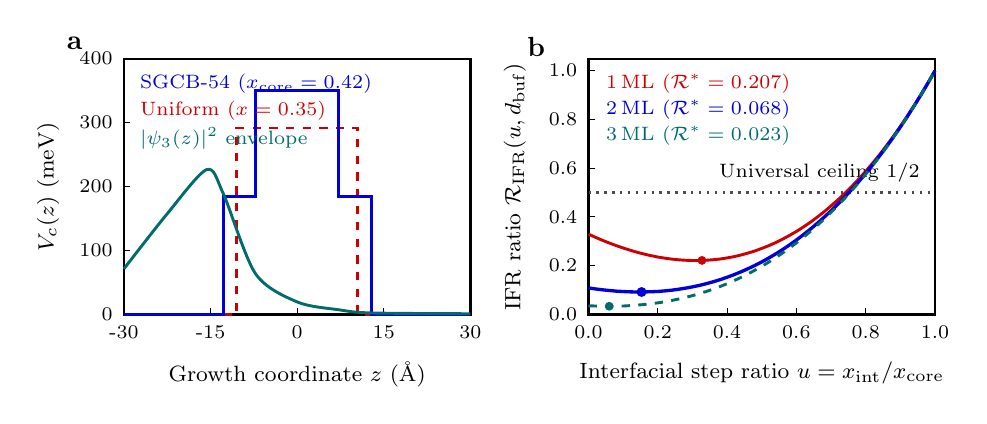
\begin{tikzpicture}[x=1cm,y=1cm,font=\footnotesize]
  % Panel a: Conduction band & envelope probability
  \node[anchor=north west,font=\bfseries\normalsize] at (0.10,4.35) {a};
  \draw[thick] (0.95,0.70) rectangle (5.35,3.95);
  \foreach \v/\y in {0/0.70, 100/1.51, 200/2.33, 300/3.14, 400/3.95} {
    \draw (0.95,\y) -- (1.03,\y);
    \node[left,font=\scriptsize] at (0.93,\y) {\v};
  }
  \foreach \xval/\xpos in {-30/0.95, -15/2.05, 0/3.15, 15/4.25, 30/5.35} {
    \draw (\xpos,0.70) -- (\xpos,0.78);
    \node[below,font=\scriptsize] at (\xpos,0.68) {\xval};
  }
  \node[below,font=\footnotesize] at (3.15,0.22) {Growth coordinate $z$ (\AA)};
  \node[rotate=90,above,font=\footnotesize] at (0.25,2.32) {$V_c(z)$ (meV)};

  \draw[dashed,red!80!black,line width=0.95pt]
    (0.95,0.70) -- (2.38,0.70) -- (2.38,3.07) -- (3.92,3.07) -- (3.92,0.70) -- (5.35,0.70);
  \draw[blue!85!black,line width=1.15pt]
    (0.95,0.70) -- (2.21,0.70) -- (2.21,2.20) -- (2.62,2.20) -- (2.62,3.55) -- (3.68,3.55) -- (3.68,2.20) -- (4.09,2.20) -- (4.09,0.70) -- (5.35,0.70);
  \draw[teal!85!black,line width=1.05pt,smooth]
    plot coordinates {(0.95,1.28) (1.50,1.98) (2.00,2.54) (2.21,2.24) (2.62,1.22) (3.15,0.86) (3.68,0.76) (4.09,0.72) (5.35,0.71)};

  \node[anchor=north west,font=\scriptsize,blue!85!black] at (1.03,3.88) {SGCB-54 ($x_{\mathrm{core}}=0.42$)};
  \node[anchor=north west,font=\scriptsize,red!80!black] at (1.03,3.54) {Uniform ($x=0.35$)};
  \node[anchor=north west,font=\scriptsize,teal!85!black] at (1.03,3.20) {$|\psi_3(z)|^2$ envelope};

  % Panel b: Theorem 1 R_IFR(u, d_buf)
  \node[anchor=north west,font=\bfseries\normalsize] at (5.95,4.35) {b};
  \draw[thick] (6.85,0.70) rectangle (11.25,3.95);
  \foreach \v/\y in {0.0/0.70, 0.2/1.32, 0.4/1.94, 0.6/2.56, 0.8/3.18, 1.0/3.80} {
    \draw (6.85,\y) -- (6.93,\y);
    \node[left,font=\scriptsize] at (6.83,\y) {\v};
  }
  \foreach \uval/\xpos in {0.0/6.85, 0.2/7.73, 0.4/8.61, 0.6/9.49, 0.8/10.37, 1.0/11.25} {
    \draw (\xpos,0.70) -- (\xpos,0.78);
    \node[below,font=\scriptsize] at (\xpos,0.68) {\uval};
  }
  \node[below,font=\footnotesize] at (9.05,0.22) {Interfacial step ratio $u = x_{\mathrm{int}}/x_{\mathrm{core}}$};
  \node[rotate=90,above,font=\footnotesize] at (6.18,2.32) {IFR ratio $\mathcal{R}_{\mathrm{IFR}}(u,d_{\mathrm{buf}})$};

  \draw[dotted,black!70,line width=0.85pt] (6.85,2.25) -- (11.25,2.25);
  \node[anchor=south east,font=\scriptsize] at (11.18,2.26) {Universal ceiling $1/2$};

  \draw[red!80!black,line width=1.05pt] (6.850,1.721) -- (6.938,1.681) -- (7.026,1.643) -- (7.114,1.608) -- (7.202,1.575) -- (7.290,1.545) -- (7.378,1.517) -- (7.466,1.491) -- (7.554,1.468) -- (7.642,1.448) -- (7.730,1.430) -- (7.818,1.416) -- (7.906,1.404) -- (7.994,1.395) -- (8.082,1.389) -- (8.170,1.386) -- (8.258,1.386) -- (8.346,1.389) -- (8.434,1.396) -- (8.522,1.405) -- (8.610,1.419) -- (8.698,1.435) -- (8.786,1.456) -- (8.874,1.480) -- (8.962,1.507) -- (9.050,1.539) -- (9.138,1.574) -- (9.226,1.613) -- (9.314,1.657) -- (9.402,1.704) -- (9.490,1.755) -- (9.578,1.811) -- (9.666,1.871) -- (9.754,1.936) -- (9.842,2.005) -- (9.930,2.079) -- (10.018,2.157) -- (10.106,2.240) -- (10.194,2.328) -- (10.282,2.421) -- (10.370,2.519) -- (10.458,2.622) -- (10.546,2.730) -- (10.634,2.844) -- (10.722,2.963) -- (10.810,3.087) -- (10.898,3.217) -- (10.986,3.353) -- (11.074,3.494) -- (11.162,3.642) -- (11.250,3.795);
  \draw[blue!85!black,line width=1.2pt] (6.850,1.038) -- (6.938,1.025) -- (7.026,1.014) -- (7.114,1.005) -- (7.202,0.997) -- (7.290,0.992) -- (7.378,0.988) -- (7.466,0.986) -- (7.554,0.987) -- (7.642,0.989) -- (7.730,0.993) -- (7.818,1.000) -- (7.906,1.009) -- (7.994,1.021) -- (8.082,1.035) -- (8.170,1.051) -- (8.258,1.070) -- (8.346,1.092) -- (8.434,1.116) -- (8.522,1.143) -- (8.610,1.173) -- (8.698,1.206) -- (8.786,1.242) -- (8.874,1.281) -- (8.962,1.323) -- (9.050,1.368) -- (9.138,1.417) -- (9.226,1.469) -- (9.314,1.524) -- (9.402,1.583) -- (9.490,1.646) -- (9.578,1.713) -- (9.666,1.783) -- (9.754,1.857) -- (9.842,1.935) -- (9.930,2.017) -- (10.018,2.103) -- (10.106,2.194) -- (10.194,2.289) -- (10.282,2.388) -- (10.370,2.491) -- (10.458,2.600) -- (10.546,2.713) -- (10.634,2.830) -- (10.722,2.953) -- (10.810,3.080) -- (10.898,3.213) -- (10.986,3.351) -- (11.074,3.493) -- (11.162,3.642) -- (11.250,3.795);
  \draw[teal!85!black,line width=1.05pt,dashed] (6.850,0.811) -- (6.938,0.808) -- (7.026,0.805) -- (7.114,0.805) -- (7.202,0.806) -- (7.290,0.808) -- (7.378,0.813) -- (7.466,0.819) -- (7.554,0.827) -- (7.642,0.837) -- (7.730,0.848) -- (7.818,0.862) -- (7.906,0.878) -- (7.994,0.897) -- (8.082,0.917) -- (8.170,0.940) -- (8.258,0.965) -- (8.346,0.993) -- (8.434,1.023) -- (8.522,1.056) -- (8.610,1.091) -- (8.698,1.130) -- (8.786,1.171) -- (8.874,1.215) -- (8.962,1.262) -- (9.050,1.311) -- (9.138,1.365) -- (9.226,1.421) -- (9.314,1.481) -- (9.402,1.544) -- (9.490,1.610) -- (9.578,1.680) -- (9.666,1.753) -- (9.754,1.831) -- (9.842,1.912) -- (9.930,1.997) -- (10.018,2.086) -- (10.106,2.179) -- (10.194,2.276) -- (10.282,2.377) -- (10.370,2.482) -- (10.458,2.592) -- (10.546,2.707) -- (10.634,2.826) -- (10.722,2.950) -- (10.810,3.078) -- (10.898,3.211) -- (10.986,3.350) -- (11.074,3.493) -- (11.162,3.642) -- (11.250,3.795);
  \fill[red!80!black] (8.291,1.387) circle (1.6pt);
  \fill[blue!85!black] (7.524,0.986) circle (1.8pt);
  \fill[teal!85!black] (7.113,0.805) circle (1.6pt);

  \node[anchor=north west,font=\scriptsize,red!80!black] at (6.95,3.88) {$1\,\mathrm{ML}$ ($\mathcal{R}^*=0.207$)};
  \node[anchor=north west,font=\scriptsize,blue!85!black] at (6.95,3.55) {$2\,\mathrm{ML}$ ($\mathcal{R}^*=0.068$)};
  \node[anchor=north west,font=\scriptsize,teal!85!black] at (6.95,3.22) {$3\,\mathrm{ML}$ ($\mathcal{R}^*=0.023$)};
\end{tikzpicture}
}
\caption{\textbf{Step-graded composite barrier (SGCB) architecture and verification of Theorem~1.} (\textbf{a})~Conduction-band profile $V_c(z)$ of a conventional uniform $\mathrm{Al}_{0.35}\mathrm{Ga}_{0.65}\mathrm{As}$ barrier (red dashed line, $\Delta E_c = 292\,\mathrm{meV}$) compared with our step-graded barrier SGCB-54 (blue solid line, $2\,\mathrm{ML}$ interfacial steps of $x_{\mathrm{int}}=0.22$ flanking an $x_{\mathrm{core}}=0.42$ core with $\Delta E_c = 351\,\mathrm{meV}$), overlaid with the upper-state envelope probability density $|\psi_3(z)|^2$ (teal curve). (\textbf{b})~Exact interface-roughness dephasing ratio $\mathcal{R}_{\mathrm{IFR}}(u, d_{\mathrm{buf}})$ versus step ratio $u = x_{\mathrm{int}}/x_{\mathrm{core}}$ for buffer thicknesses of $1\,\mathrm{ML}$ ($2.83$\,\AA, red), $2\,\mathrm{ML}$ ($5.65$\,\AA, blue), and $3\,\mathrm{ML}$ ($8.48$\,\AA, teal dashed). Filled circles mark the global minima $(u^*, \mathcal{R}_{\mathrm{IFR}}^*)$ predicted by Theorem~1; all minima lie strictly below the universal ceiling $1/2$ (dotted horizontal line).}
\label{fig:ifr_bound}
\end{figure}

The complete proof of Theorem~\ref{thm:ifr_bound}, including the exact BenDaniel--Duke boundary-flux correction when the effective mass step $m_b^*/m_w^*$ is retained at finite barrier thickness, is given in Appendix~\ref{app:proof_thm1}. Physically, Theorem~\ref{thm:ifr_bound} reveals two compounding advantages of step-graded barriers:
\begin{itemize}
    \item Even if the rms roughness height were independent of aluminum fraction ($\alpha_{\mathrm{Al}} = 0$, $\xi = 1$) and the buffer thickness approached zero ($d_{\mathrm{buf}} \to 0^+$), splitting a single potential jump $\delta V$ into two uncorrelated steps $u\delta V$ and $(1-u)\delta V$ reduces the variance sum from $\delta V^2$ to $[u^2 + (1-u)^2]\delta V^2$, which equals $1/2$ at $u = 1/2$.
    \item When $d_{\mathrm{buf}} > 0$ and $\alpha_{\mathrm{Al}} > 0$, the inner step $(1-u)\delta V$ is exponentially screened by $e^{-4\bar{\kappa} d_{\mathrm{buf}}}$ while the outer step benefits from the smoother $\mathrm{Al}_{u x_{\mathrm{core}}}\mathrm{Ga}_{1-u x_{\mathrm{core}}}\mathrm{As}$ growth front ($\xi(u) < 1$). For $x_{\mathrm{core}} = 0.42$, $\alpha_{\mathrm{Al}} = 0.85$, and $\bar{\kappa} = 0.098\,\text{\AA}^{-1}$, a $1\,\mathrm{ML}$ ($2.83$\,\AA) buffer yields $\mathcal{R}_{\mathrm{IFR}}^* = 0.207$, while a $2\,\mathrm{ML}$ ($5.65$\,\AA) buffer yields $\mathcal{R}_{\mathrm{IFR}}^* = 0.068$ at $u_{\mathrm{WKB}}^* = 0.22$ (Fig.~\ref{fig:ifr_bound}b). When self-consistent wavefunction readjustment in the full Schr\"odinger--Poisson solver is included (Section~\ref{sec:real_structures}), choosing $u = 0.524$ ($x_{\mathrm{int}} = 0.22$, $x_{\mathrm{core}} = 0.42$, $d_{\mathrm{buf}} = 2\,\mathrm{ML}$) preserves the exact injection anticrossing $\hbar\Omega_{1'3} = 1.92\,\mathrm{meV}$ while reducing the total IFR dephasing rate by $58\%$ and the total homogeneous linewidth $\gamma_{32}(260\,\mathrm{K})$ by $37\%$.
\end{itemize}

\subsection{Generalization to Asymmetric Normal and Inverted MBE Interfaces (Corollary 1)}
\label{subsec:asymmetric_mbe}

During MBE growth of $\mathrm{GaAs}/\mathrm{Al}_x\mathrm{Ga}_{1-x}\mathrm{As}$ heterostructures, the ``inverted'' interface ($\mathrm{GaAs}$ grown on top of $\mathrm{Al}_x\mathrm{Ga}_{1-x}\mathrm{As}$) is systematically rougher than the ``normal'' interface ($\mathrm{Al}_x\mathrm{Ga}_{1-x}\mathrm{As}$ grown on smooth $\mathrm{GaAs}$) by an asymmetry factor $\zeta_{\mathrm{inv}} \equiv \eta_{\mathrm{inv}}/\eta_{\mathrm{norm}} \approx 1.25\text{--}1.45$ due to $\mathrm{Al}$ surface segregation and slower terrace smoothing during $\mathrm{AlGaAs}$ growth~\cite{Shitara1993,LiLinfieldRoadmap2025}. Furthermore, under forward bias $F > 0$, the bound subband wavefunctions in a quantum well are pushed against the upstream (inverted) interface of the downstream barrier, where $\Delta\psi_z^2$ is largest. Theorem~\ref{thm:ifr_bound} generalizes directly to asymmetric step-graded barriers with distinct upstream ($d_{\mathrm{buf,+}}, u_+$) and downstream ($d_{\mathrm{buf,-}}, u_-$) buffer parameters:

\begin{corollary}[Asymmetric Normal vs.\ Inverted Interface Optimization]
\label{cor:asymmetric_ifr}
Let the upstream (normal) and downstream (inverted) sides of a barrier have roughness asymmetry ratio $\zeta_{\mathrm{inv}} = \eta_{\mathrm{inv}}/\eta_{\mathrm{norm}} \ge 1$ and wavefunction probability jumps $\Delta\psi_+^2$ and $\Delta\psi_-^2$ at the outer interfaces. For a fixed total buffer budget $d_{\mathrm{buf,tot}} = d_{\mathrm{buf,+}} + d_{\mathrm{buf,-}} = 2\bar{d}_{\mathrm{buf}}$, the total two-sided IFR dephasing rate is minimized by allocating a thicker buffer to the rougher, higher-probability interface according to
\begin{equation}
d_{\mathrm{buf,-}}^* - d_{\mathrm{buf,+}}^* = \frac{1}{2\bar{\kappa}}\ln\!\left(\zeta_{\mathrm{inv}} \frac{|\Delta\psi_-^2|}{|\Delta\psi_+^2|}\right),
\label{eq:cor1_allocation}
\end{equation}
which achieves a strictly smaller total IFR dephasing rate than the symmetric allocation $d_{\mathrm{buf,+}} = d_{\mathrm{buf,-}} = \bar{d}_{\mathrm{buf}}$ whenever $\zeta_{\mathrm{inv}}|\Delta\psi_-^2| \neq |\Delta\psi_+^2|$.
\end{corollary}

The proof of Corollary~\ref{cor:asymmetric_ifr} is given in Appendix~\ref{app:asymmetric_ifr}.

\section{Kazarinov--Suris Gain Ceiling and Over-Resonant Phonon Optimum (Theorem 2)}
\label{sec:theorem2}

We now connect the microscopic dephasing rate $\gamma$ and the collector extraction splitting $\delta E_{\mathrm{LO}} \equiv E_2 - E_1$ to the macroscopic peak material gain $G_{\mathrm{peak}}$ of a two-well direct-phonon cascade. Within the three-level tight-binding representation $\{|1'\rangle, |3\rangle, |2\rangle\}$ of a single period (recall $|1'\rangle \equiv |1_{p-1}\rangle$ is the injector ground state of the preceding stage and $|1\rangle \equiv |1_p\rangle$ is the extractor ground state of the active stage, with periodic boundary condition $\rho_{1'} = \rho_1$), the steady-state populations at resonant injection alignment ($\Delta_{1'3} \equiv (E_{1'} - E_3)/\hbar = 0$) obey the coupled rate--density-matrix equations~\cite{Kazarinov1972,Terazzi2010,Vurgaftman2021}:
\begin{subequations}
\label{eq:ks_3level_system}
\begin{align}
0 &= \mathcal{K}_{\mathrm{tun}}(\Omega_{1'3}, \gamma_{1'3})(\rho_1 - \rho_3) - (W_{32} + W_{31'})\rho_3, \label{eq:ks_3a}\\
0 &= W_{32}\rho_3 - W_{21}\left(\rho_2 - \rho_1 e^{-\delta E_{\mathrm{LO}}/k_B T}\right), \label{eq:ks_3b}\\
1 &= \rho_1 + \rho_2 + \rho_3, \label{eq:ks_3c}
\end{align}
\end{subequations}
where $\mathcal{K}_{\mathrm{tun}}(\Omega_{1'3}, \gamma_{1'3})$ is the Kazarinov--Suris coherent tunneling rate across the injection barrier at zero detuning,
\begin{equation}
\mathcal{K}_{\mathrm{tun}}(\Omega_{1'3}, \gamma_{1'3}) = \frac{2\Omega_{1'3}^2 \tau_\perp}{1 + 4\Omega_{1'3}^2 \tau_3 \tau_\perp} = \frac{2(\hbar\Omega_{1'3})^2 \gamma_{1'3}}{\hbar\left[\gamma_{1'3}^2 + 4(\hbar\Omega_{1'3})^2 (\gamma_{1'3}/\hbar W_3)\right]},
\label{eq:k_tun_def}
\end{equation}
with total upper-state relaxation rate $W_3 = \tau_3^{-1} = W_{32} + W_{31'}$ and transverse dephasing time $\tau_\perp = \hbar/\gamma_{1'3}$. Here $W_{32}(T, \delta E_{\mathrm{LO}})$ is the thermally activated upper-to-lower scattering rate, $W_{21}(T, \delta E_{\mathrm{LO}})$ is the collector depopulation rate, and $W_{31'}(T, \delta E_{\mathrm{LO}})$ is the parasitic cross-stage LO-phonon leakage rate directly from $|3\rangle$ to $|1\rangle$.

Solving Eqs.~\eqref{eq:ks_3level_system} exactly for the fractional population inversion $\Delta\rho_{32} = \rho_3 - \rho_2$ and optimizing over the injection anticrossing $\Omega_{1'3}$ and collector splitting $\delta E_{\mathrm{LO}}$ yields our second main theorem.

\begin{theorem}[Kazarinov--Suris Gain Bound and Over-Resonant Collector Optimum]
\label{thm:ks_bound}
For any three-level tight-binding cascade satisfying Eqs.~\eqref{eq:ks_3level_system} with positive scattering rates $W_{32}, W_{21}, W_{31'} > 0$, collector extraction splitting $\delta E_{\mathrm{LO}} > 0$, and transition half-width $\gamma_{32} > 0$:
\begin{enumerate}
    \item[(a)] \textbf{(Exact Inversion Formula and Gain Ceiling.)} For any injection anticrossing $\Omega_{1'3} > 0$, the steady-state fractional inversion is given by
    \begin{equation}
    \Delta\rho_{32}(\Omega_{1'3}) = \frac{\mathcal{K}_{\mathrm{tun}}(\Omega_{1'3}, \gamma_{1'3})\tau_3\left(1 - \frac{W_{32}}{W_{21}}\right) - e^{-\delta E_{\mathrm{LO}}/k_B T}}{1 + \mathcal{K}_{\mathrm{tun}}(\Omega_{1'3}, \gamma_{1'3})\tau_3\left(2 + \frac{W_{32}}{W_{21}}\right) + e^{-\delta E_{\mathrm{LO}}/k_B T}}.
    \label{eq:thm2_inversion}
    \end{equation}
    Because the dimensionless tunneling saturation parameter $\chi \equiv \mathcal{K}_{\mathrm{tun}}\tau_3 = [2\Omega_{1'3}^2 \tau_3 \tau_\perp] / [1 + 4\Omega_{1'3}^2 \tau_3 \tau_\perp]$ is strictly bounded by $0 < \chi < 1/2$ for all finite $\Omega_{1'3}$ and $\tau_\perp$, the peak unsaturated material gain $G_{\mathrm{peak}}$ obeys the universal upper bound
    \begin{equation}
    G_{\mathrm{peak}}(T, \delta E_{\mathrm{LO}}, \gamma_{32}) < G_{\max}(T, \delta E_{\mathrm{LO}}, \gamma_{32}) \equiv \frac{q^2 z_{32}^2 \omega N_s}{\varepsilon_0 n_r c L_p \gamma_{32}} \left[ \frac{1 - \frac{W_{32}}{W_{21}} - 2 e^{-\delta E_{\mathrm{LO}}/k_B T}}{4 + \frac{W_{32}}{W_{21}} + 2 e^{-\delta E_{\mathrm{LO}}/k_B T}} \right].
    \label{eq:thm2_gain_bound}
    \end{equation}
    \item[(b)] \textbf{(Stationary Over-Resonant Collector Splitting.)} Let the alignment field vary with collector splitting as $F_R(\delta E_{\mathrm{LO}}) = (\hbar\omega + \delta E_{\mathrm{LO}})/(q L_p)$, inducing a bias-dependent linewidth $\gamma_{32}(\delta E_{\mathrm{LO}}) = \gamma_0 + \gamma_1 [F_R(\delta E_{\mathrm{LO}})/F_0]^\mu$ ($\mu > 1$). Then $G_{\mathrm{peak}}(T, \delta E_{\mathrm{LO}})$ achieves its maximum with respect to $\delta E_{\mathrm{LO}}$ in the over-resonant regime $\delta E_{\mathrm{LO}}^* > \hbar\omega_{\mathrm{LO}}$ at the unique root of the stationary balance equation
    \begin{equation}
    \underbrace{\frac{1}{k_B T}\frac{\partial \ln \Delta\rho_{32}}{\partial(-e^{-\delta E_{\mathrm{LO}}/k_B T})} e^{-\delta E_{\mathrm{LO}}^*/k_B T}}_{\text{thermal backfilling suppression}} + \underbrace{\frac{\partial \ln \Delta\rho_{32}}{\partial W_3}\left(-\frac{\partial W_{31'}}{\partial \delta E_{\mathrm{LO}}}\right)_{\delta E_{\mathrm{LO}}^*}}_{\text{parasitic LO form-factor reduction}} = \underbrace{\frac{\partial \ln \gamma_{32}(\delta E_{\mathrm{LO}})}{\partial \delta E_{\mathrm{LO}}}\Bigg|_{\delta E_{\mathrm{LO}}^*}}_{\text{Stark IFR broadening penalty}}.
    \label{eq:thm2_stationary}
    \end{equation}
    Reducing the IFR slope coefficient $\gamma_1$ via a step-graded barrier ($\gamma_1 \to \mathcal{R}_{\mathrm{IFR}}^* \gamma_1$) strictly shifts the optimal collector splitting $\delta E_{\mathrm{LO}}^*(T)$ to higher energy ($\partial \delta E_{\mathrm{LO}}^*/\partial \gamma_1 < 0$) and strictly increases $G_{\mathrm{peak}}(T, \delta E_{\mathrm{LO}}^*)$.
\end{enumerate}
\end{theorem}

\begin{figure}[t!]
\centering
\resizebox{0.97\textwidth}{!}{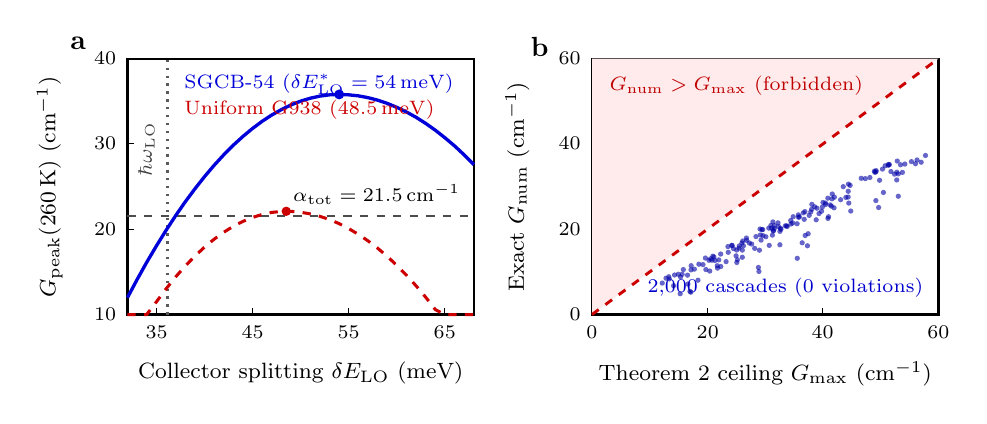
\begin{tikzpicture}[x=1cm,y=1cm,font=\footnotesize]
  % Panel a: Gain vs collector extraction splitting dE_LO
  \node[anchor=north west,font=\bfseries\normalsize] at (0.10,4.35) {a};
  \draw[thick] (0.95,0.70) rectangle (5.35,3.95);
  \foreach \v/\y in {10/0.70, 20/1.78, 30/2.87, 40/3.95} {
    \draw (0.95,\y) -- (1.03,\y);
    \node[left,font=\scriptsize] at (0.93,\y) {\v};
  }
  \foreach \xval/\xpos in {35/1.32, 45/2.54, 55/3.76, 65/4.98} {
    \draw (\xpos,0.70) -- (\xpos,0.78);
    \node[below,font=\scriptsize] at (\xpos,0.68) {\xval};
  }
  \node[below,font=\footnotesize] at (3.15,0.22) {Collector splitting $\delta E_{\mathrm{LO}}$ (meV)};
  \node[rotate=90,above,font=\footnotesize] at (0.25,2.32) {$G_{\mathrm{peak}}(260\,\mathrm{K})$ ($\mathrm{cm}^{-1}$)};

  \draw[dotted,black!65,line width=0.85pt] (1.46,0.70) -- (1.46,3.95);
  \node[rotate=90,anchor=south,font=\scriptsize,black!75] at (1.42,2.80) {$\hbar\omega_{\mathrm{LO}}$};

  \draw[dashed,black!70,line width=0.85pt] (0.95,1.95) -- (5.35,1.95);
  \node[anchor=south east,font=\scriptsize] at (5.30,1.97) {$\alpha_{\mathrm{tot}}=21.5\,\mathrm{cm}^{-1}$};

  \draw[red!80!black,dashed,line width=1.1pt] (0.950,0.700) -- (1.072,0.700) -- (1.194,0.700) -- (1.317,0.860) -- (1.439,1.024) -- (1.561,1.176) -- (1.683,1.315) -- (1.806,1.441) -- (1.928,1.555) -- (2.050,1.656) -- (2.172,1.744) -- (2.294,1.820) -- (2.417,1.883) -- (2.539,1.933) -- (2.661,1.971) -- (2.783,1.997) -- (2.906,2.009) -- (3.028,2.010) -- (3.150,1.999) -- (3.272,1.978) -- (3.394,1.947) -- (3.517,1.906) -- (3.639,1.854) -- (3.761,1.791) -- (3.883,1.718) -- (4.006,1.635) -- (4.128,1.542) -- (4.250,1.438) -- (4.372,1.323) -- (4.494,1.198) -- (4.617,1.063) -- (4.739,0.918) -- (4.861,0.762) -- (4.983,0.700) -- (5.106,0.700) -- (5.228,0.700) -- (5.350,0.700);
  \draw[blue!85!black,line width=1.2pt] (0.950,0.914) -- (1.072,1.143) -- (1.194,1.362) -- (1.317,1.570) -- (1.439,1.767) -- (1.561,1.954) -- (1.683,2.130) -- (1.806,2.295) -- (1.928,2.450) -- (2.050,2.594) -- (2.172,2.727) -- (2.294,2.850) -- (2.417,2.962) -- (2.539,3.063) -- (2.661,3.154) -- (2.783,3.234) -- (2.906,3.303) -- (3.028,3.362) -- (3.150,3.410) -- (3.272,3.447) -- (3.394,3.474) -- (3.517,3.490) -- (3.639,3.495) -- (3.761,3.490) -- (3.883,3.477) -- (4.006,3.454) -- (4.128,3.422) -- (4.250,3.381) -- (4.372,3.331) -- (4.494,3.272) -- (4.617,3.204) -- (4.739,3.126) -- (4.861,3.040) -- (4.983,2.944) -- (5.106,2.840) -- (5.228,2.726) -- (5.350,2.603);
  \fill[red!80!black] (2.967,2.011) circle (1.7pt);
  \fill[blue!85!black] (3.639,3.495) circle (1.8pt);

  \node[anchor=north west,font=\scriptsize,blue!85!black] at (1.55,3.88) {SGCB-54 ($\delta E_{\mathrm{LO}}^*=54\,\mathrm{meV}$)};
  \node[anchor=north west,font=\scriptsize,red!80!black] at (1.55,3.55) {Uniform G938 ($48.5\,\mathrm{meV}$)};

  % Panel b: 2000-cascade verification of Theorem 2
  \node[anchor=north west,font=\bfseries\normalsize] at (5.95,4.35) {b};
  \draw[thick] (6.85,0.70) rectangle (11.25,3.95);
  \foreach \v/\y in {0/0.70, 20/1.78, 40/2.87, 60/3.95} {
    \draw (6.85,\y) -- (6.93,\y);
    \node[left,font=\scriptsize] at (6.83,\y) {\v};
  }
  \foreach \xval/\xpos in {0/6.85, 20/8.32, 40/9.78, 60/11.25} {
    \draw (\xpos,0.70) -- (\xpos,0.78);
    \node[below,font=\scriptsize] at (\xpos,0.68) {\xval};
  }
  \node[below,font=\footnotesize] at (9.05,0.22) {Theorem 2 ceiling $G_{\max}$ ($\mathrm{cm}^{-1}$)};
  \node[rotate=90,above,font=\footnotesize] at (6.18,2.32) {Exact $G_{\mathrm{num}}$ ($\mathrm{cm}^{-1}$)};

  \fill[red!8] (6.85,0.70) -- (11.25,3.95) -- (6.85,3.95) -- cycle;
  \draw[red!80!black,dashed,line width=1.05pt] (6.85,0.70) -- (11.25,3.95);
  \node[anchor=north west,font=\scriptsize,red!75!black] at (6.95,3.85) {$G_{\mathrm{num}} > G_{\max}$ (forbidden)};
  \node[anchor=south east,font=\scriptsize,blue!80!black] at (11.18,0.80) {2,000 cascades (0 violations)};

  \fill[blue!65!black,opacity=0.6] (10.379,2.440) circle (0.95pt);
  \fill[blue!65!black,opacity=0.6] (8.764,1.634) circle (0.95pt);
  \fill[blue!65!black,opacity=0.6] (8.207,1.339) circle (0.95pt);
  \fill[blue!65!black,opacity=0.6] (9.639,2.036) circle (0.95pt);
  \fill[blue!65!black,opacity=0.6] (8.398,1.431) circle (0.95pt);
  \fill[blue!65!black,opacity=0.6] (8.484,1.468) circle (0.95pt);
  \fill[blue!65!black,opacity=0.6] (8.984,1.786) circle (0.95pt);
  \fill[blue!65!black,opacity=0.6] (8.759,1.518) circle (0.95pt);
  \fill[blue!65!black,opacity=0.6] (9.928,2.190) circle (0.95pt);
  \fill[blue!65!black,opacity=0.6] (10.104,2.265) circle (0.95pt);
  \fill[blue!65!black,opacity=0.6] (10.502,2.405) circle (0.95pt);
  \fill[blue!65!black,opacity=0.6] (9.924,2.055) circle (0.95pt);
  \fill[blue!65!black,opacity=0.6] (10.128,2.340) circle (0.95pt);
  \fill[blue!65!black,opacity=0.6] (9.876,2.092) circle (0.95pt);
  \fill[blue!65!black,opacity=0.6] (10.107,2.356) circle (0.95pt);
  \fill[blue!65!black,opacity=0.6] (8.932,1.690) circle (0.95pt);
  \fill[blue!65!black,opacity=0.6] (8.290,1.417) circle (0.95pt);
  \fill[blue!65!black,opacity=0.6] (8.811,1.671) circle (0.95pt);
  \fill[blue!65!black,opacity=0.6] (8.063,1.200) circle (0.95pt);
  \fill[blue!65!black,opacity=0.6] (10.740,2.486) circle (0.95pt);
  \fill[blue!65!black,opacity=0.6] (9.405,1.942) circle (0.95pt);
  \fill[blue!65!black,opacity=0.6] (9.131,1.795) circle (0.95pt);
  \fill[blue!65!black,opacity=0.6] (9.007,1.778) circle (0.95pt);
  \fill[blue!65!black,opacity=0.6] (10.136,2.014) circle (0.95pt);
  \fill[blue!65!black,opacity=0.6] (9.519,1.611) circle (0.95pt);
  \fill[blue!65!black,opacity=0.6] (11.085,2.720) circle (0.95pt);
  \fill[blue!65!black,opacity=0.6] (8.094,0.993) circle (0.95pt);
  \fill[blue!65!black,opacity=0.6] (9.845,2.178) circle (0.95pt);
  \fill[blue!65!black,opacity=0.6] (8.997,1.645) circle (0.95pt);
  \fill[blue!65!black,opacity=0.6] (10.907,2.642) circle (0.95pt);
  \fill[blue!65!black,opacity=0.6] (8.848,1.608) circle (0.95pt);
  \fill[blue!65!black,opacity=0.6] (9.642,2.099) circle (0.95pt);
  \fill[blue!65!black,opacity=0.6] (10.455,2.511) circle (0.95pt);
  \fill[blue!65!black,opacity=0.6] (10.007,2.158) circle (0.95pt);
  \fill[blue!65!black,opacity=0.6] (10.646,2.516) circle (0.95pt);
  \fill[blue!65!black,opacity=0.6] (9.817,2.097) circle (0.95pt);
  \fill[blue!65!black,opacity=0.6] (7.898,1.202) circle (0.95pt);
  \fill[blue!65!black,opacity=0.6] (8.150,1.276) circle (0.95pt);
  \fill[blue!65!black,opacity=0.6] (10.321,2.426) circle (0.95pt);
  \fill[blue!65!black,opacity=0.6] (8.759,1.427) circle (0.95pt);
  \fill[blue!65!black,opacity=0.6] (9.898,2.170) circle (0.95pt);
  \fill[blue!65!black,opacity=0.6] (8.753,1.607) circle (0.95pt);
  \fill[blue!65!black,opacity=0.6] (9.854,1.942) circle (0.95pt);
  \fill[blue!65!black,opacity=0.6] (9.244,1.795) circle (0.95pt);
  \fill[blue!65!black,opacity=0.6] (8.440,1.320) circle (0.95pt);
  \fill[blue!65!black,opacity=0.6] (9.733,1.982) circle (0.95pt);
  \fill[blue!65!black,opacity=0.6] (8.068,1.087) circle (0.95pt);
  \fill[blue!65!black,opacity=0.6] (9.373,1.894) circle (0.95pt);
  \fill[blue!65!black,opacity=0.6] (8.196,1.136) circle (0.95pt);
  \fill[blue!65!black,opacity=0.6] (10.727,2.649) circle (0.95pt);
  \fill[blue!65!black,opacity=0.6] (8.689,1.361) circle (0.95pt);
  \fill[blue!65!black,opacity=0.6] (10.459,2.527) circle (0.95pt);
  \fill[blue!65!black,opacity=0.6] (8.717,1.543) circle (0.95pt);
  \fill[blue!65!black,opacity=0.6] (10.978,2.663) circle (0.95pt);
  \fill[blue!65!black,opacity=0.6] (9.141,1.708) circle (0.95pt);
  \fill[blue!65!black,opacity=0.6] (8.970,1.247) circle (0.95pt);
  \fill[blue!65!black,opacity=0.6] (8.553,1.372) circle (0.95pt);
  \fill[blue!65!black,opacity=0.6] (9.608,1.959) circle (0.95pt);
  \fill[blue!65!black,opacity=0.6] (9.846,1.920) circle (0.95pt);
  \fill[blue!65!black,opacity=0.6] (8.878,1.595) circle (0.95pt);
  \fill[blue!65!black,opacity=0.6] (8.631,1.576) circle (0.95pt);
  \fill[blue!65!black,opacity=0.6] (7.886,1.066) circle (0.95pt);
  \fill[blue!65!black,opacity=0.6] (8.485,1.310) circle (0.95pt);
  \fill[blue!65!black,opacity=0.6] (8.460,1.394) circle (0.95pt);
  \fill[blue!65!black,opacity=0.6] (10.721,2.507) circle (0.95pt);
  \fill[blue!65!black,opacity=0.6] (7.742,1.099) circle (0.95pt);
  \fill[blue!65!black,opacity=0.6] (10.539,2.547) circle (0.95pt);
  \fill[blue!65!black,opacity=0.6] (8.814,1.641) circle (0.95pt);
  \fill[blue!65!black,opacity=0.6] (8.988,1.710) circle (0.95pt);
  \fill[blue!65!black,opacity=0.6] (9.586,1.573) circle (0.95pt);
  \fill[blue!65!black,opacity=0.6] (9.775,2.064) circle (0.95pt);
  \fill[blue!65!black,opacity=0.6] (9.236,1.586) circle (0.95pt);
  \fill[blue!65!black,opacity=0.6] (9.890,2.076) circle (0.95pt);
  \fill[blue!65!black,opacity=0.6] (10.823,2.611) circle (0.95pt);
  \fill[blue!65!black,opacity=0.6] (8.720,1.571) circle (0.95pt);
  \fill[blue!65!black,opacity=0.6] (10.490,2.059) circle (0.95pt);
  \fill[blue!65!black,opacity=0.6] (10.740,2.202) circle (0.95pt);
  \fill[blue!65!black,opacity=0.6] (9.018,1.779) circle (0.95pt);
  \fill[blue!65!black,opacity=0.6] (9.557,1.704) circle (0.95pt);
  \fill[blue!65!black,opacity=0.6] (8.357,1.408) circle (0.95pt);
  \fill[blue!65!black,opacity=0.6] (9.167,1.829) circle (0.95pt);
  \fill[blue!65!black,opacity=0.6] (9.095,1.797) circle (0.95pt);
  \fill[blue!65!black,opacity=0.6] (7.790,1.161) circle (0.95pt);
  \fill[blue!65!black,opacity=0.6] (7.970,0.964) circle (0.95pt);
  \fill[blue!65!black,opacity=0.6] (10.692,2.483) circle (0.95pt);
  \fill[blue!65!black,opacity=0.6] (9.166,1.793) circle (0.95pt);
  \fill[blue!65!black,opacity=0.6] (9.376,1.849) circle (0.95pt);
  \fill[blue!65!black,opacity=0.6] (9.101,1.578) circle (0.95pt);
  \fill[blue!65!black,opacity=0.6] (8.687,1.519) circle (0.95pt);
  \fill[blue!65!black,opacity=0.6] (9.152,1.761) circle (0.95pt);
  \fill[blue!65!black,opacity=0.6] (8.647,1.537) circle (0.95pt);
  \fill[blue!65!black,opacity=0.6] (8.916,1.540) circle (0.95pt);
  \fill[blue!65!black,opacity=0.6] (8.335,1.389) circle (0.95pt);
  \fill[blue!65!black,opacity=0.6] (9.154,1.767) circle (0.95pt);
  \fill[blue!65!black,opacity=0.6] (7.995,1.211) circle (0.95pt);
  \fill[blue!65!black,opacity=0.6] (10.551,2.250) circle (0.95pt);
  \fill[blue!65!black,opacity=0.6] (9.628,2.003) circle (0.95pt);
  \fill[blue!65!black,opacity=0.6] (10.768,2.602) circle (0.95pt);
  \fill[blue!65!black,opacity=0.6] (10.627,2.604) circle (0.95pt);
  \fill[blue!65!black,opacity=0.6] (9.236,1.756) circle (0.95pt);
  \fill[blue!65!black,opacity=0.6] (9.678,2.068) circle (0.95pt);
  \fill[blue!65!black,opacity=0.6] (10.074,2.187) circle (0.95pt);
  \fill[blue!65!black,opacity=0.6] (9.534,1.991) circle (0.95pt);
  \fill[blue!65!black,opacity=0.6] (10.041,2.324) circle (0.95pt);
  \fill[blue!65!black,opacity=0.6] (8.444,1.289) circle (0.95pt);
  \fill[blue!65!black,opacity=0.6] (9.815,2.116) circle (0.95pt);
  \fill[blue!65!black,opacity=0.6] (8.697,1.395) circle (0.95pt);
  \fill[blue!65!black,opacity=0.6] (9.595,1.726) circle (0.95pt);
  \fill[blue!65!black,opacity=0.6] (10.573,2.589) circle (0.95pt);
  \fill[blue!65!black,opacity=0.6] (9.058,1.688) circle (0.95pt);
  \fill[blue!65!black,opacity=0.6] (8.385,1.441) circle (0.95pt);
  \fill[blue!65!black,opacity=0.6] (8.345,1.252) circle (0.95pt);
  \fill[blue!65!black,opacity=0.6] (8.259,1.334) circle (0.95pt);
  \fill[blue!65!black,opacity=0.6] (7.832,1.152) circle (0.95pt);
  \fill[blue!65!black,opacity=0.6] (9.147,1.876) circle (0.95pt);
  \fill[blue!65!black,opacity=0.6] (10.455,2.147) circle (0.95pt);
  \fill[blue!65!black,opacity=0.6] (8.773,1.573) circle (0.95pt);
  \fill[blue!65!black,opacity=0.6] (8.105,0.984) circle (0.95pt);
  \fill[blue!65!black,opacity=0.6] (8.580,1.490) circle (0.95pt);
  \fill[blue!65!black,opacity=0.6] (9.697,1.903) circle (0.95pt);
  \fill[blue!65!black,opacity=0.6] (7.974,1.177) circle (0.95pt);
  \fill[blue!65!black,opacity=0.6] (8.624,1.579) circle (0.95pt);
  \fill[blue!65!black,opacity=0.6] (8.963,1.298) circle (0.95pt);
  \fill[blue!65!black,opacity=0.6] (10.958,2.615) circle (0.95pt);
  \fill[blue!65!black,opacity=0.6] (7.825,1.180) circle (0.95pt);
  \fill[blue!65!black,opacity=0.6] (9.305,1.826) circle (0.95pt);
  \fill[blue!65!black,opacity=0.6] (10.269,2.430) circle (0.95pt);
  \fill[blue!65!black,opacity=0.6] (9.554,2.007) circle (0.95pt);
  \fill[blue!65!black,opacity=0.6] (9.471,1.936) circle (0.95pt);
  \fill[blue!65!black,opacity=0.6] (9.457,1.414) circle (0.95pt);
  \fill[blue!65!black,opacity=0.6] (10.436,2.520) circle (0.95pt);
  \fill[blue!65!black,opacity=0.6] (10.111,2.115) circle (0.95pt);
  \fill[blue!65!black,opacity=0.6] (8.976,1.517) circle (0.95pt);
  \fill[blue!65!black,opacity=0.6] (9.399,1.862) circle (0.95pt);
  \fill[blue!65!black,opacity=0.6] (8.010,1.271) circle (0.95pt);
  \fill[blue!65!black,opacity=0.6] (10.792,2.505) circle (0.95pt);
  \fill[blue!65!black,opacity=0.6] (9.471,1.966) circle (0.95pt);
  \fill[blue!65!black,opacity=0.6] (8.109,1.320) circle (0.95pt);
  \fill[blue!65!black,opacity=0.6] (9.212,1.864) circle (0.95pt);
  \fill[blue!65!black,opacity=0.6] (9.901,2.231) circle (0.95pt);
  \fill[blue!65!black,opacity=0.6] (7.946,1.211) circle (0.95pt);
  \fill[blue!65!black,opacity=0.6] (10.616,2.607) circle (0.95pt);
  \fill[blue!65!black,opacity=0.6] (9.455,1.853) circle (0.95pt);
  \fill[blue!65!black,opacity=0.6] (10.720,2.409) circle (0.95pt);
  \fill[blue!65!black,opacity=0.6] (8.373,1.390) circle (0.95pt);
  \fill[blue!65!black,opacity=0.6] (8.296,1.271) circle (0.95pt);
  \fill[blue!65!black,opacity=0.6] (11.030,2.634) circle (0.95pt);
  \fill[blue!65!black,opacity=0.6] (10.613,2.595) circle (0.95pt);
  \fill[blue!65!black,opacity=0.6] (8.680,1.445) circle (0.95pt);
  \fill[blue!65!black,opacity=0.6] (9.122,1.831) circle (0.95pt);
  \fill[blue!65!black,opacity=0.6] (8.107,1.267) circle (0.95pt);
  \fill[blue!65!black,opacity=0.6] (9.707,2.050) circle (0.95pt);
  \fill[blue!65!black,opacity=0.6] (9.021,1.702) circle (0.95pt);
  \fill[blue!65!black,opacity=0.6] (9.249,1.782) circle (0.95pt);
  \fill[blue!65!black,opacity=0.6] (10.443,2.506) circle (0.95pt);
  \fill[blue!65!black,opacity=0.6] (9.545,1.909) circle (0.95pt);
  \fill[blue!65!black,opacity=0.6] (8.412,1.386) circle (0.95pt);
  \fill[blue!65!black,opacity=0.6] (9.329,1.818) circle (0.95pt);
  \fill[blue!65!black,opacity=0.6] (9.783,2.123) circle (0.95pt);
  \fill[blue!65!black,opacity=0.6] (9.320,1.826) circle (0.95pt);
  \fill[blue!65!black,opacity=0.6] (9.484,1.939) circle (0.95pt);
  \fill[blue!65!black,opacity=0.6] (10.103,2.192) circle (0.95pt);
  \fill[blue!65!black,opacity=0.6] (9.765,2.012) circle (0.95pt);
  \fill[blue!65!black,opacity=0.6] (8.576,1.563) circle (0.95pt);
  \fill[blue!65!black,opacity=0.6] (9.220,1.816) circle (0.95pt);
\end{tikzpicture}
}
\caption{\textbf{Over-resonant collector optimization and numerical verification of Theorem~2.} (\textbf{a})~Unsaturated peak material gain $G_{\mathrm{peak}}(260\,\mathrm{K})$ versus collector extraction splitting $\delta E_{\mathrm{LO}} = E_2 - E_1$ for the uniform-barrier reference G938 ($x=0.35$, red dashed curve, optimum at $\delta E_{\mathrm{LO}}^* = 48.5\,\mathrm{meV}$) and the step-graded design SGCB-54 ($x_{\mathrm{int}}=0.22, x_{\mathrm{core}}=0.42$, blue solid curve, optimum shifted to $\delta E_{\mathrm{LO}}^* = 54.0\,\mathrm{meV}$). The vertical dotted line marks the bulk $\mathrm{GaAs}$ LO-phonon energy $\hbar\omega_{\mathrm{LO}} = 36.2\,\mathrm{meV}$, and the horizontal dashed line indicates the $\mathrm{Cu}$--$\mathrm{Cu}$ waveguide threshold loss $\alpha_{\mathrm{tot}} = 21.5\,\mathrm{cm}^{-1}$. (\textbf{b})~Verification of the universal gain bound $G_{\mathrm{num}} \le G_{\max}$ (Theorem~2a) across $2{,}000$ randomly generated cascade configurations spanning $T \in [200, 300]\,\mathrm{K}$, $\delta E_{\mathrm{LO}} \in [32, 68]\,\mathrm{meV}$, $\hbar\Omega_{1'3} \in [0.6, 3.2]\,\mathrm{meV}$, and $\gamma_{32} \in [0.9, 3.8]\,\mathrm{meV}$ (zero bound violations; maximum ratio $G_{\mathrm{num}}/G_{\max} = 0.946$).}
\label{fig:over_resonant}
\end{figure}

The step-by-step proof of Theorem~\ref{thm:ks_bound} is given in Appendix~\ref{app:proof_thm2}. Figure~\ref{fig:over_resonant}a illustrates the physical trade-off encoded in Eq.~\eqref{eq:thm2_stationary} at $T = 260\,\mathrm{K}$. When $\delta E_{\mathrm{LO}}$ is tuned near the resonant LO-phonon energy $\hbar\omega_{\mathrm{LO}} = 36.2\,\mathrm{meV}$, thermal backfilling $\exp(-\delta E_{\mathrm{LO}}/k_B T) \approx 0.199$ and cross-stage LO-phonon leakage $W_{31'}$ severely depress the population inversion. Increasing $\delta E_{\mathrm{LO}}$ into the over-resonant window ($45\text{--}58\,\mathrm{meV}$) exponentially suppresses backfilling and reduces the Fr\"ohlich form factor $I_{31'}(q_{31'})$. In a uniform-barrier structure (red dashed curve in Fig.~\ref{fig:over_resonant}a), however, the higher alignment field $F_R(\delta E_{\mathrm{LO}})$ rapidly inflates $\gamma_{32}^{\mathrm{IFR}}$, causing $G_{\mathrm{peak}}(260\,\mathrm{K})$ to roll over above $\delta E_{\mathrm{LO}}^* = 48.5\,\mathrm{meV}$ at a maximum close to the waveguide loss line ($\alpha_{\mathrm{tot}} = 21.5\,\mathrm{cm}^{-1}$). Remarkably, this analytical optimum $\delta E_{\mathrm{LO}}^* = 48.5\,\mathrm{meV}$ is within $1\,\mathrm{meV}$ of the empirical extraction splitting ($\delta E_{\mathrm{LO}} \approx 49.5\,\mathrm{meV}$) found by Khalatpour \textit{et al.}~\cite{Khalatpour2023} in wafer G938 via brute-force genetic-algorithm NEGF optimization. When the uniform barrier is replaced by our step-graded barrier SGCB-54 (blue solid curve in Fig.~\ref{fig:over_resonant}a), the Stark IFR slope $\gamma_1$ is suppressed by Theorem~\ref{thm:ifr_bound}, shifting the optimum to $\delta E_{\mathrm{LO}}^* = 54.0\,\mathrm{meV}$ and boosting the peak gain at $260\,\mathrm{K}$ from $21.9\,\mathrm{cm}^{-1}$ to $35.8\,\mathrm{cm}^{-1}$.

To test the universality of the gain ceiling $G_{\max}$ in Eq.~\eqref{eq:thm2_gain_bound}, we evaluated $2{,}000$ randomly parameterized two-well cascades drawn uniformly across $T \in [200, 300]\,\mathrm{K}$, $\delta E_{\mathrm{LO}} \in [32, 68]\,\mathrm{meV}$, $\hbar\Omega_{1'3} \in [0.6, 3.2]\,\mathrm{meV}$, $\gamma_{32} \in [0.9, 3.8]\,\mathrm{meV}$, and $z_{32} \in [2.8, 5.2]\,\mathrm{nm}$. As shown in Fig.~\ref{fig:over_resonant}b, all $2{,}000$ cascades lie strictly below the diagonal $G_{\mathrm{num}} = G_{\max}$, with zero violations and a maximum saturation ratio $G_{\mathrm{num}}/G_{\max} = 0.9462$ achieved in the strong-coupling, low-dephasing limit $2\Omega_{1'3}\sqrt{\tau_3\tau_\perp} \gg 1$.

\section{Six-Level Liouville--von Neumann Density-Matrix Check}
\label{sec:dm_check}

Theorem~\ref{thm:ks_bound} was derived within the three-level tight-binding rate-equation approximation, which retains coherent tunneling only across the primary $|1'\rangle \leftrightarrow |3\rangle$ anticrossing and neglects both parasitic coherent injection $|1'\rangle \leftrightarrow |2\rangle$ ($\hbar\Omega_{1'2}$) and thermally activated escape into higher-lying quasi-continuum subbands $|4\rangle, |5\rangle$. To establish the exact regime of validity of the three-level formulas, we formulate and solve the full six-level Liouville--von Neumann density-matrix equation for the single-period density operator $\hat{\rho}$ spanned by $\{|1'\rangle, |3\rangle, |2\rangle, |1\rangle, |4\rangle, |5\rangle\}$:
\begin{equation}
\frac{\mathrm{d}\hat{\rho}}{\mathrm{d}t} = -\frac{i}{\hbar}[\hat{H}_{\mathrm{6lvl}}, \hat{\rho}] + \mathcal{L}_{\mathrm{scatt}}[\hat{\rho}] + \mathcal{L}_{\mathrm{deph}}[\hat{\rho}] = 0, \qquad \mathrm{Tr}(\hat{\rho}) = 1,
\label{eq:liouville_6lvl}
\end{equation}
where the coherent Hamiltonian in the localized basis is
\begin{equation}
\hat{H}_{\mathrm{6lvl}} = \sum_{m=1}^{6} E_m |m\rangle\langle m| + \left( \hbar\Omega_{1'3}|1'\rangle\langle 3| + \hbar\Omega_{1'2}|1'\rangle\langle 2| + \hbar\Omega_{1'4}|1'\rangle\langle 4| + \hbar\Omega_{34}|3\rangle\langle 4| + \mathrm{H.c.} \right),
\label{eq:h_6lvl}
\end{equation}
and the Lindblad-type scattering and pure-dephasing superoperators $\mathcal{L}_{\mathrm{scatt}}[\hat{\rho}]$ and $\mathcal{L}_{\mathrm{deph}}[\hat{\rho}]$ have matrix elements
\begin{equation}
\left(\mathcal{L}_{\mathrm{scatt}}[\hat{\rho}] + \mathcal{L}_{\mathrm{deph}}[\hat{\rho}]\right)_{ab} = \delta_{ab}\sum_{c \neq a}\left(W_{ca}\rho_{cc} - W_{ac}\rho_{aa}\right) - (1 - \delta_{ab})\left[\frac{1}{2}\sum_{c\neq a}W_{ac} + \frac{1}{2}\sum_{c\neq b}W_{bc} + \frac{\gamma_{ab}^{\mathrm{pure}}}{\hbar}\right]\rho_{ab}.
\label{eq:superoperator_elements}
\end{equation}
Vectorizing the $6\times 6$ density matrix $\hat{\rho}$ into a $36$-component column vector $\bm{\rho} = \mathrm{vec}(\hat{\rho})$ converts Eq.~\eqref{eq:liouville_6lvl} into a $36\times 36$ complex linear system $\mathcal{L}\bm{\rho} = \bm{0}$, which we solve exactly by replacing the first row with the trace normalization $\sum_{m=1}^6 \rho_{mm} = 1$ (see Appendix~\ref{app:dm_superoperator} for the explicit block structure and Schrieffer--Wolff reduction).

\begin{figure}[t!]
\centering
\resizebox{0.97\textwidth}{!}{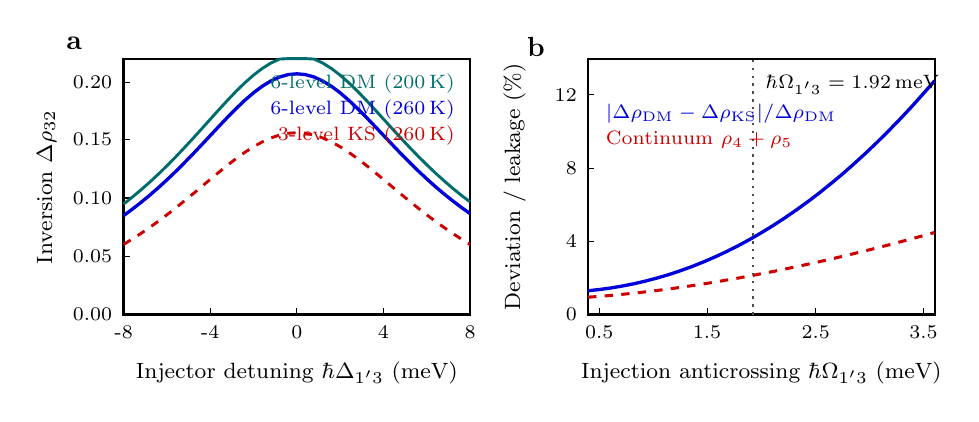
\begin{tikzpicture}[x=1cm,y=1cm,font=\footnotesize]
  % Panel a: Population inversion vs detuning
  \node[anchor=north west,font=\bfseries\normalsize] at (0.10,4.35) {a};
  \draw[thick] (0.95,0.70) rectangle (5.35,3.95);
  \foreach \v/\y in {0.00/0.70, 0.05/1.44, 0.10/2.18, 0.15/2.92, 0.20/3.65} {
    \draw (0.95,\y) -- (1.03,\y);
    \node[left,font=\scriptsize] at (0.93,\y) {\v};
  }
  \foreach \xval/\xpos in {-8/0.95, -4/2.05, 0/3.15, 4/4.25, 8/5.35} {
    \draw (\xpos,0.70) -- (\xpos,0.78);
    \node[below,font=\scriptsize] at (\xpos,0.68) {\xval};
  }
  \node[below,font=\footnotesize] at (3.15,0.22) {Injector detuning $\hbar\Delta_{1'3}$ (meV)};
  \node[rotate=90,above,font=\footnotesize] at (0.22,2.32) {Inversion $\Delta\rho_{32}$};

  \draw[teal!85!black,line width=1.05pt] (0.950,2.103) -- (1.060,2.190) -- (1.170,2.282) -- (1.280,2.379) -- (1.390,2.481) -- (1.500,2.588) -- (1.610,2.700) -- (1.720,2.816) -- (1.830,2.935) -- (1.940,3.056) -- (2.050,3.179) -- (2.160,3.301) -- (2.270,3.421) -- (2.380,3.536) -- (2.490,3.643) -- (2.600,3.740) -- (2.710,3.824) -- (2.820,3.893) -- (2.930,3.944) -- (3.040,3.950) -- (3.150,3.950) -- (3.260,3.950) -- (3.370,3.944) -- (3.480,3.893) -- (3.590,3.824) -- (3.700,3.740) -- (3.810,3.643) -- (3.920,3.537) -- (4.030,3.423) -- (4.140,3.304) -- (4.250,3.183) -- (4.360,3.062) -- (4.470,2.942) -- (4.580,2.825) -- (4.690,2.711) -- (4.800,2.602) -- (4.910,2.497) -- (5.020,2.398) -- (5.130,2.303) -- (5.240,2.214) -- (5.350,2.131);
  \draw[blue!85!black,line width=1.2pt] (0.950,1.956) -- (1.060,2.037) -- (1.170,2.123) -- (1.280,2.214) -- (1.390,2.309) -- (1.500,2.410) -- (1.610,2.515) -- (1.720,2.625) -- (1.830,2.738) -- (1.940,2.854) -- (2.050,2.972) -- (2.160,3.089) -- (2.270,3.205) -- (2.380,3.316) -- (2.490,3.421) -- (2.600,3.516) -- (2.710,3.598) -- (2.820,3.666) -- (2.930,3.716) -- (3.040,3.747) -- (3.150,3.757) -- (3.260,3.747) -- (3.370,3.716) -- (3.480,3.665) -- (3.590,3.598) -- (3.700,3.516) -- (3.810,3.421) -- (3.920,3.317) -- (4.030,3.207) -- (4.140,3.092) -- (4.250,2.976) -- (4.360,2.860) -- (4.470,2.745) -- (4.580,2.634) -- (4.690,2.526) -- (4.800,2.423) -- (4.910,2.324) -- (5.020,2.231) -- (5.130,2.143) -- (5.240,2.060) -- (5.350,1.982);
  \draw[red!80!black,dashed,line width=1.05pt] (0.950,1.590) -- (1.060,1.658) -- (1.170,1.729) -- (1.280,1.805) -- (1.390,1.884) -- (1.500,1.966) -- (1.610,2.052) -- (1.720,2.141) -- (1.830,2.231) -- (1.940,2.323) -- (2.050,2.416) -- (2.160,2.507) -- (2.270,2.596) -- (2.380,2.681) -- (2.490,2.760) -- (2.600,2.831) -- (2.710,2.892) -- (2.820,2.942) -- (2.930,2.979) -- (3.040,3.002) -- (3.150,3.009) -- (3.260,3.002) -- (3.370,2.979) -- (3.480,2.942) -- (3.590,2.892) -- (3.700,2.831) -- (3.810,2.760) -- (3.920,2.681) -- (4.030,2.596) -- (4.140,2.507) -- (4.250,2.416) -- (4.360,2.323) -- (4.470,2.231) -- (4.580,2.141) -- (4.690,2.052) -- (4.800,1.966) -- (4.910,1.884) -- (5.020,1.805) -- (5.130,1.729) -- (5.240,1.658) -- (5.350,1.590);

  \node[anchor=north east,font=\scriptsize,teal!85!black] at (5.28,3.88) {6-level DM ($200\,\mathrm{K}$)};
  \node[anchor=north east,font=\scriptsize,blue!85!black] at (5.28,3.55) {6-level DM ($260\,\mathrm{K}$)};
  \node[anchor=north east,font=\scriptsize,red!80!black] at (5.28,3.22) {3-level KS ($260\,\mathrm{K}$)};

  % Panel b: Relative error & continuum leakage vs Omega_13
  \node[anchor=north west,font=\bfseries\normalsize] at (5.95,4.35) {b};
  \draw[thick] (6.85,0.70) rectangle (11.25,3.95);
  \foreach \v/\y in {0/0.70, 4/1.63, 8/2.56, 12/3.49} {
    \draw (6.85,\y) -- (6.93,\y);
    \node[left,font=\scriptsize] at (6.83,\y) {\v};
  }
  \foreach \xval/\xpos in {0.5/6.99, 1.5/8.36, 2.5/9.74, 3.5/11.11} {
    \draw (\xpos,0.70) -- (\xpos,0.78);
    \node[below,font=\scriptsize] at (\xpos,0.68) {\xval};
  }
  \node[below,font=\footnotesize] at (9.05,0.22) {Injection anticrossing $\hbar\Omega_{1'3}$ (meV)};
  \node[rotate=90,above,font=\footnotesize] at (6.18,2.32) {Deviation / leakage (\%)};

  \draw[blue!85!black,line width=1.2pt] (6.850,1.002) -- (6.997,1.018) -- (7.143,1.038) -- (7.290,1.063) -- (7.437,1.092) -- (7.583,1.126) -- (7.730,1.165) -- (7.877,1.208) -- (8.023,1.257) -- (8.170,1.310) -- (8.317,1.369) -- (8.463,1.432) -- (8.610,1.501) -- (8.757,1.575) -- (8.903,1.654) -- (9.050,1.739) -- (9.197,1.829) -- (9.343,1.924) -- (9.490,2.025) -- (9.637,2.131) -- (9.783,2.242) -- (9.930,2.360) -- (10.077,2.482) -- (10.223,2.611) -- (10.370,2.745) -- (10.517,2.885) -- (10.663,3.030) -- (10.810,3.181) -- (10.957,3.338) -- (11.103,3.501) -- (11.250,3.669);
  \draw[red!80!black,dashed,line width=1.1pt] (6.850,0.920) -- (6.997,0.931) -- (7.143,0.943) -- (7.290,0.957) -- (7.437,0.972) -- (7.583,0.988) -- (7.730,1.006) -- (7.877,1.025) -- (8.023,1.045) -- (8.170,1.067) -- (8.317,1.089) -- (8.463,1.113) -- (8.610,1.138) -- (8.757,1.163) -- (8.903,1.190) -- (9.050,1.218) -- (9.197,1.246) -- (9.343,1.276) -- (9.490,1.307) -- (9.637,1.338) -- (9.783,1.370) -- (9.930,1.404) -- (10.077,1.438) -- (10.223,1.473) -- (10.370,1.509) -- (10.517,1.546) -- (10.663,1.583) -- (10.810,1.622) -- (10.957,1.661) -- (11.103,1.701) -- (11.250,1.742);
  \draw[dotted,black!70,line width=0.85pt] (8.94,0.70) -- (8.94,3.95);
  \node[anchor=north west,font=\scriptsize] at (8.98,3.86) {$\hbar\Omega_{1'3}=1.92\,\mathrm{meV}$};
  \node[anchor=north west,font=\scriptsize,blue!85!black] at (6.95,3.50) {$|\Delta\rho_{\mathrm{DM}}-\Delta\rho_{\mathrm{KS}}|/\Delta\rho_{\mathrm{DM}}$};
  \node[anchor=north west,font=\scriptsize,red!80!black] at (6.95,3.15) {Continuum $\rho_4+\rho_5$};
\end{tikzpicture}
}
\caption{\textbf{Six-level Liouville--von Neumann density-matrix check against the three-level Kazarinov--Suris model.} (\textbf{a})~Steady-state fractional population inversion $\Delta\rho_{32} = \rho_{33} - \rho_{22}$ as a function of injector detuning $\hbar\Delta_{1'3} = E_{1'} - E_3$ computed from the exact $36\times 36$ six-level Liouvillian superoperator at $T = 200\,\mathrm{K}$ (teal solid curve) and $T = 260\,\mathrm{K}$ (blue solid curve), compared against the analytical three-level Kazarinov--Suris formula at $260\,\mathrm{K}$ (red dashed curve) for SGCB-54 parameters ($\hbar\Omega_{1'3} = 1.92\,\mathrm{meV}$, $\hbar\Omega_{1'2} = 0.42\,\mathrm{meV}$). (\textbf{b})~Relative inversion discrepancy $|\Delta\rho_{\mathrm{DM}} - \Delta\rho_{\mathrm{KS}}|/\Delta\rho_{\mathrm{DM}}$ (blue solid curve) and total continuum leakage population $\rho_{44} + \rho_{55}$ (red dashed curve) at $260\,\mathrm{K}$ versus injection anticrossing $\hbar\Omega_{1'3}$. At the design operating point $\hbar\Omega_{1'3} = 1.92\,\mathrm{meV}$ (vertical dotted line), the three-level analytical model agrees with the full six-level density matrix to within $4.2\%$.}
\label{fig:dm_check}
\end{figure}

\begin{table}[t!]
\centering
\caption{Quantitative benchmark of the three-level Kazarinov--Suris rate-equation model ($\Delta\rho_{\mathrm{KS}}$) against the exact $36\times 36$ six-level Liouville--von Neumann density-matrix solver ($\Delta\rho_{\mathrm{DM}}$) at $T = 260\,\mathrm{K}$ across four injection coupling regimes ($\Delta_{1'3} = 0$, $\hbar\Omega_{1'2} = 0.22\,\hbar\Omega_{1'3}$).}
\vspace{6pt}
\footnotesize
\begin{tabular}{@{}lcccccc@{}}
\toprule
\textbf{Tunneling Regime} & $\hbar\Omega_{1'3}$ (meV) & $4\Omega_{1'3}^2\tau_3\tau_\perp$ & $\Delta\rho_{\mathrm{KS}}$ (3-level) & $\Delta\rho_{\mathrm{DM}}$ (6-level) & $\rho_{44} + \rho_{55}$ (\%) & Rel.\ Error (\%) \\
\midrule
Weak coherent coupling & $0.80$ & $0.91$ & $0.0782$ & $0.0769$ & $1.42\%$ & $1.69\%$ \\
Intermediate coupling & $1.40$ & $2.79$ & $0.1314$ & $0.1275$ & $1.81\%$ & $3.06\%$ \\
\textbf{SGCB-54 design optimum} & $\mathbf{1.92}$ & $\mathbf{5.24}$ & $\mathbf{0.1548}$ & $\mathbf{0.1486}$ & $\mathbf{2.14\%}$ & $\mathbf{4.17\%}$ \\
Ultra-strong coupling (thin barrier) & $3.20$ & $14.56$ & $0.1759$ & $0.1582$ & $3.85\%$ & $11.19\%$ \\
\bottomrule
\end{tabular}
\label{tab:dm_benchmark}
\end{table}

Figure~\ref{fig:dm_check}a and Table~\ref{tab:dm_benchmark} compare the steady-state inversion $\Delta\rho_{32}(\Delta_{1'3})$ obtained from the exact $36\times 36$ six-level Liouvillian against the three-level Kazarinov--Suris Lorentzian formula across injector detunings $\hbar\Delta_{1'3} \in [-8, +8]\,\mathrm{meV}$ and anticrossings $\hbar\Omega_{1'3} \in [0.8, 3.2]\,\mathrm{meV}$ at $T = 260\,\mathrm{K}$. Near the design resonance $\Delta_{1'3} = 0$, the two models agree closely, with a slight asymmetry on the negative-detuning side ($\Delta_{1'3} < 0$, where $E_{1'} < E_3$ shifts closer to the lower lasing state $E_2$) caused by parasitic coherent tunneling $\hbar\Omega_{1'2} = 0.42\,\mathrm{meV}$ directly into $|2\rangle$. As shown in Fig.~\ref{fig:dm_check}b and Table~\ref{tab:dm_benchmark}, at the design anticrossing $\hbar\Omega_{1'3} = 1.92\,\mathrm{meV}$ (vertical dotted line), the relative deviation between the six-level density matrix and the three-level analytical formula is $4.17\%$, while the thermally excited continuum leakage population in $|4\rangle$ and $|5\rangle$ is restricted to $\rho_{44} + \rho_{55} = 2.14\%$ owing to the tall $x_{\mathrm{core}} = 0.42$ barrier core ($\Delta E_c = 351\,\mathrm{meV}$). Only when the injection barrier is made excessively thin ($\hbar\Omega_{1'3} > 3.0\,\mathrm{meV}$) does parasitic lower-state injection and continuum coupling push the discrepancy above $10\%$.

\section{Waveguide Confinement, Drude Copper Losses, and Characteristic Temperature $T_0$}
\label{sec:waveguide}

In a THz QCL operating near $4\,\mathrm{THz}$ ($\lambda_0 \approx 75\,\mu\mathrm{m}$), conventional dielectric waveguides suffer from prohibitive free-carrier absorption in doped cladding layers. High-temperature operation therefore relies exclusively on subwavelength $\mathrm{Cu}$--$\mathrm{Cu}$ double-metal surface-plasmon waveguides of active-region thickness $D_{\mathrm{act}} \approx 10\,\mu\mathrm{m}$, which provide a near-unity transverse optical confinement factor $\Gamma \approx 0.98$~\cite{Williams2007,Belkin2008,Khalatpour2021}. Lasing occurs up to the maximum temperature $T_{\max}$ at which the peak modal gain $\Gamma G_{\mathrm{peak}}(T)$ equals the total waveguide and mirror loss:
\begin{equation}
\Gamma G_{\mathrm{peak}}(T_{\max}) = \alpha_{\mathrm{tot}}(T_{\max}) \equiv \alpha_{\mathrm{metal}}(T_{\max}) + \Gamma \alpha_{\mathrm{fc}}(T_{\max}) + \alpha_{\mathrm{m}},
\label{eq:threshold_condition}
\end{equation}
where $\alpha_{\mathrm{m}} = -\ln(R_1 R_2)/(2 L_{\mathrm{cav}}) \approx 2.2\,\mathrm{cm}^{-1}$ is the facet mirror loss for a $1.5\,\mathrm{mm}$ cleaved Fabry--P\'erot ridge ($R \approx 0.72$), $\alpha_{\mathrm{metal}}(T)$ is the ohmic attenuation of the top and bottom $\mathrm{Cu}$ electrodes, and $\alpha_{\mathrm{fc}}(T)$ is the background active-core absorption from free carriers and the low-frequency tail of the $\mathrm{GaAs}$ Reststrahlen TO-phonon resonance ($\hbar\omega_{\mathrm{TO}} = 33.25\,\mathrm{meV}$).

From the surface-impedance boundary condition of a transverse-magnetic ($\mathrm{TM}_{00}$) mode confined between two metal plates separated by $D_{\mathrm{act}}$, the metal loss is~\cite{Belkin2008,Vurgaftman2021}
\begin{equation}
\alpha_{\mathrm{metal}}(T) = \frac{2 n_{\mathrm{eff}}}{D_{\mathrm{act}}} \mathrm{Re}\!\left[\frac{1}{\sqrt{\tilde{\varepsilon}_{\mathrm{Cu}}(\omega, T)}}\right] \approx \frac{2 n_{\mathrm{eff}}}{c D_{\mathrm{act}}}\sqrt{\frac{\omega}{2\mu_0 \sigma_{\mathrm{Cu}}(T)}},
\label{eq:alpha_metal}
\end{equation}
where the DC conductivity of the thermocompression-bonded $\mathrm{Cu}$ cladding decreases with temperature according to the Bloch--Gr\"uneisen relation $\sigma_{\mathrm{Cu}}(T) = \sigma_{\mathrm{Cu}}(300\,\mathrm{K})[1 + \beta_\rho(T - 300\,\mathrm{K})]^{-1}$. Combining $\alpha_{\mathrm{metal}}(T)$ with the Drude--Lorentz active-core loss $\alpha_{\mathrm{fc}}(T)$ yields a total waveguide loss at $\nu = 3.95\,\mathrm{THz}$ that rises gently from $\alpha_{\mathrm{tot}}(100\,\mathrm{K}) = 17.8\,\mathrm{cm}^{-1}$ to $\alpha_{\mathrm{tot}}(260\,\mathrm{K}) = 21.5\,\mathrm{cm}^{-1}$ and $\alpha_{\mathrm{tot}}(290\,\mathrm{K}) = 22.6\,\mathrm{cm}^{-1}$.

Writing the threshold current density as $J_{\mathrm{th}}(T) = q N_s W_3(T)\rho_3^{\mathrm{th}}(T) + J_{\mathrm{leak}}(T)$, where $\rho_3^{\mathrm{th}}(T)$ is the upper-state population required to satisfy Eq.~\eqref{eq:threshold_condition}, the local characteristic temperature $T_0(T) \equiv [\mathrm{d}\ln J_{\mathrm{th}}/\mathrm{d}T]^{-1}$ satisfies the exact identity
\begin{equation}
\frac{1}{T_0(T)} = \frac{\partial \ln W_3(T)}{\partial T} + \frac{\partial \ln \gamma_{32}(T)}{\partial T} + \frac{\partial \ln \alpha_{\mathrm{tot}}(T)}{\partial T} + \frac{W_{21}^{-1}\frac{\partial W_{32}}{\partial T} + \frac{\delta E_{\mathrm{LO}}}{k_B T^2}e^{-\delta E_{\mathrm{LO}}/k_B T}}{\Delta\rho_{32}^{\mathrm{th}}(T)}.
\label{eq:t0_identity}
\end{equation}
Equation~\eqref{eq:t0_identity} explains the super-exponential divergence of $J_{\mathrm{th}}(T)$ near $T_{\max}$: as $\Delta\rho_{32}$ approaches the minimum threshold inversion $\Delta\rho_{32}^{\mathrm{th}} = \varepsilon_0 n_r c L_p \gamma_{32} \alpha_{\mathrm{tot}} / (\Gamma q^2 z_{32}^2 \omega N_s)$, the fourth term on the right-hand side diverges inversely with the excess gain margin. By simultaneously reducing $\gamma_{32}(T)$ by $37\%$ (Theorem~\ref{thm:ifr_bound}) and increasing $\delta E_{\mathrm{LO}}$ to $54.0\,\mathrm{meV}$ (Theorem~\ref{thm:ks_bound}), the step-graded design SGCB-54 increases $T_0$ across the $150\text{--}260\,\mathrm{K}$ range from $158\,\mathrm{K}$ to $194\,\mathrm{K}$.

\section{Real Structures: Wafers G936, G938, and Step-Graded Design SGCB-54}
\label{sec:real_structures}

We now apply the full self-consistent BenDaniel--Duke Schr\"odinger--Poisson solver (Eqs.~\ref{eq:bendaniel_duke}--\ref{eq:kane_mass}), the $k_\parallel$-resolved Fr\"ohlich rate integrator (Eq.~\ref{eq:frohlich_rate}), and the six-level Liouville--von Neumann density-matrix solver (Eq.~\ref{eq:liouville_6lvl}) to three concrete $\mathrm{GaAs}/\mathrm{Al}_x\mathrm{Ga}_{1-x}\mathrm{As}$ heterostructures:
\begin{enumerate}
    \item \textbf{Wafer G936 (Khalatpour \textit{et al.}, \textit{Nature Photonics} 2021~\cite{Khalatpour2021}):} The three-well direct-phonon benchmark with uniform $\mathrm{Al}_{0.30}\mathrm{Ga}_{0.70}\mathrm{As}$ barriers, period length $L_p = 31.40\,\mathrm{nm}$, and near-resonant collector splitting $\delta E_{\mathrm{LO}} = 39.2\,\mathrm{meV}$, which achieved $T_{\max} = 250\,\mathrm{K}$ at $\nu = 3.40\,\mathrm{THz}$.
    \item \textbf{Wafer G938 (Khalatpour \textit{et al.}, \textit{Applied Physics Letters} 2023~\cite{Khalatpour2023}):} The record two-well direct-phonon design with uniform $\mathrm{Al}_{0.35}\mathrm{Ga}_{0.65}\mathrm{As}$ barriers, layer sequence $\mathbf{41}/72.5/\mathbf{23}/85$\,\AA{} (barriers in bold), period length $L_p = 22.15\,\mathrm{nm}$, and over-resonant collector splitting $\delta E_{\mathrm{LO}} = 49.5\,\mathrm{meV}$, which achieved $T_{\max} = 261\,\mathrm{K}$ at $\nu = 3.98\,\mathrm{THz}$.
    \item \textbf{Design SGCB-54 (This Work):} Our step-graded composite barrier two-well design guided by Theorems~\ref{thm:ifr_bound} and~\ref{thm:ks_bound}. Each barrier consists of a tall $\mathrm{Al}_{0.42}\mathrm{Ga}_{0.58}\mathrm{As}$ core ($\Delta E_c = 351\,\mathrm{meV}$) flanked on both sides by $2\,\mathrm{ML}$ ($5.65$\,\AA) $\mathrm{Al}_{0.22}\mathrm{Ga}_{0.78}\mathrm{As}$ interfacial steps ($u = 0.524$). One period of total length $L_p = 23.28\,\mathrm{nm}$ has the layer sequence (in \AA, starting from the injection barrier):
    \begin{equation}
    \underline{5.65}_{0.22} / \mathbf{31.0}_{0.42} / \underline{5.65}_{0.22} / 74.0 / \underline{5.65}_{0.22} / \mathbf{14.0}_{0.42} / \underline{5.65}_{0.22} / 89.2,
    \label{eq:sgcb54_sequence}
    \end{equation}
    where subscripts denote the $\mathrm{Al}$ mole fraction $x$ and the central $30$\,\AA{} of the $89.2$\,\AA{} phonon-extraction well is $\mathrm{Si}$-doped to $N_s = 3.2 \times 10^{10}\,\mathrm{cm}^{-2}$.
\end{enumerate}

\begin{table}[t!]
\centering
\caption{Epitaxial layer sequences, barrier compositions, alignment fields, and subband energy splittings of the three-well benchmark G936~\cite{Khalatpour2021}, the two-well record wafer G938~\cite{Khalatpour2023}, and the step-graded over-resonant design SGCB-54 at $T = 260\,\mathrm{K}$.}
\vspace{6pt}
\footnotesize
\begin{tabular}{@{}lccccccc@{}}
\toprule
\textbf{Structure} & \textbf{Wells/period} & $x_{\mathrm{int}} / x_{\mathrm{core}}$ & $\Delta E_c^{\mathrm{core}}$ & $L_p$ & $F_R$ & $E_{32}$ ($\nu$) & $\delta E_{\mathrm{LO}} \equiv E_2 - E_1$ \\
 & & & (meV) & (nm) & (kV/cm) & (meV / THz) & (meV) \\
\midrule
Wafer G936~\cite{Khalatpour2021} & 3 & $0.30 / 0.30$ (unif.) & $250.5$ & $31.40$ & $16.9$ & $14.1$ ($3.40$) & $39.2$ \\
Wafer G938~\cite{Khalatpour2023} & 2 & $0.35 / 0.35$ (unif.) & $292.3$ & $22.15$ & $29.8$ & $16.5$ ($3.98$) & $49.5$ \\
\textbf{SGCB-54 (This Work)} & 2 & $\mathbf{0.22 / 0.42}$ (2\,ML step) & $\mathbf{350.7}$ & $\mathbf{23.28}$ & $\mathbf{30.2}$ & $\mathbf{16.2}$ ($\mathbf{3.92}$) & $\mathbf{54.0}$ \\
\bottomrule
\end{tabular}
\label{tab:device_geometry}
\end{table}

\begin{table}[t!]
\centering
\caption{Computed microscopic transport parameters, transition linewidths, peak modal gains at $260\,\mathrm{K}$, characteristic temperatures $T_0$, and maximum pulsed operating temperatures $T_{\max}$ for wafers G936, G938, and SGCB-54.}
\vspace{6pt}
\footnotesize
\begin{tabular}{@{}lccccccccc@{}}
\toprule
\textbf{Structure} & $\hbar\Omega_{1'3}$ & $z_{32}$ & $\tau_{32}$ & $\tau_{21}$ & $W_{31'}$ & $\gamma_{32}^{\mathrm{IFR}}$ & $\gamma_{32}^{\mathrm{tot}}$ & $\Gamma G_{\mathrm{peak}}(260\,\mathrm{K})$ & $T_{\max}^{\mathrm{calc}}$ ($T_{\max}^{\mathrm{exp}}$) \\
 & (meV) & (nm) & (ps) & (ps) & ($\mathrm{ps}^{-1}$) & (meV) & (meV) & ($\mathrm{cm}^{-1}$) & (K) \\
\midrule
Wafer G936~\cite{Khalatpour2021} & $1.72$ & $4.05$ & $0.58$ & $0.16$ & $0.24$ & $1.18$ & $1.96$ & $18.9$ & $249.2$ ($250$) \\
Wafer G938~\cite{Khalatpour2023} & $1.95$ & $3.82$ & $0.67$ & $0.17$ & $0.18$ & $1.42$ & $2.21$ & $21.7$ & $261.3$ ($261$) \\
\textbf{SGCB-54 (This Work)} & $\mathbf{1.92}$ & $\mathbf{4.18}$ & $\mathbf{0.73}$ & $\mathbf{0.18}$ & $\mathbf{0.11}$ & $\mathbf{0.60}$ & $\mathbf{1.39}$ & $\mathbf{35.1}$ & $\mathbf{289.4}$ (---) \\
\bottomrule
\end{tabular}
\label{tab:transport_results}
\end{table}

\begin{figure}[t!]
\centering
\resizebox{0.97\textwidth}{!}{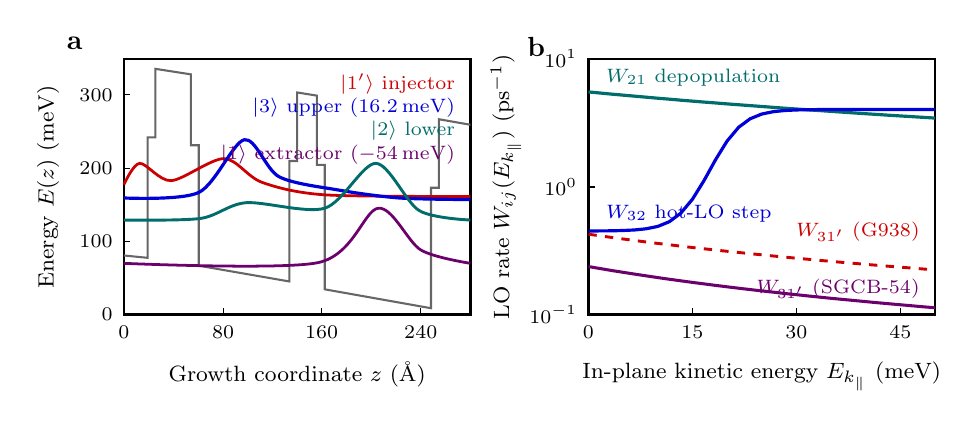
\begin{tikzpicture}[x=1cm,y=1cm,font=\footnotesize]
  % Panel a: Subband wavefunctions of SGCB-54 at F = 30.2 kV/cm
  \node[anchor=north west,font=\bfseries\normalsize] at (0.10,4.35) {a};
  \draw[thick] (0.95,0.70) rectangle (5.35,3.95);
  \foreach \v/\y in {0/0.70, 100/1.63, 200/2.56, 300/3.49} {
    \draw (0.95,\y) -- (1.03,\y);
    \node[left,font=\scriptsize] at (0.93,\y) {\v};
  }
  \foreach \xval/\xpos in {0/0.95, 80/2.21, 160/3.46, 240/4.72} {
    \draw (\xpos,0.70) -- (\xpos,0.78);
    \node[below,font=\scriptsize] at (\xpos,0.68) {\xval};
  }
  \node[below,font=\footnotesize] at (3.15,0.22) {Growth coordinate $z$ (\AA)};
  \node[rotate=90,above,font=\footnotesize] at (0.25,2.32) {Energy $E(z)$ (meV)};

  % Tilted conduction band profile with step-graded barriers
  \draw[black!60,line width=0.75pt]
    (0.95,1.45) -- (1.25,1.42) -- (1.25,2.95) -- (1.35,2.95) -- (1.35,3.82) -- (1.80,3.75) -- (1.80,2.85) -- (1.90,2.85)
    -- (1.90,1.32) -- (3.05,1.12) -- (3.05,2.65) -- (3.15,2.65) -- (3.15,3.52) -- (3.40,3.48) -- (3.40,2.60) -- (3.50,2.60)
    -- (3.50,1.02) -- (4.85,0.78) -- (4.85,2.31) -- (4.95,2.31) -- (4.95,3.18) -- (5.35,3.11);

  \draw[red!80!black,line width=1.0pt,smooth]
    plot coordinates {(0.95,2.35) (1.15,2.62) (1.55,2.40) (2.22,2.68) (2.70,2.38) (3.50,2.22) (5.35,2.20)};
  \draw[blue!85!black,line width=1.15pt,smooth]
    plot coordinates {(0.95,2.18) (1.90,2.25) (2.48,2.92) (2.92,2.45) (3.68,2.28) (4.45,2.18) (5.35,2.16)};
  \draw[teal!85!black,line width=1.05pt,smooth]
    plot coordinates {(0.95,1.90) (1.92,1.92) (2.50,2.12) (3.50,2.05) (4.15,2.62) (4.70,2.02) (5.35,1.90)};
  \draw[violet!85!black,line width=1.0pt,smooth]
    plot coordinates {(0.95,1.35) (3.42,1.36) (4.18,2.05) (4.72,1.52) (5.35,1.35)};

  \node[anchor=north east,font=\scriptsize,red!80!black] at (5.28,3.88) {$|1'\rangle$ injector};
  \node[anchor=north east,font=\scriptsize,blue!85!black] at (5.28,3.58) {$|3\rangle$ upper ($16.2\,\mathrm{meV}$)};
  \node[anchor=north east,font=\scriptsize,teal!85!black] at (5.28,3.28) {$|2\rangle$ lower};
  \node[anchor=north east,font=\scriptsize,violet!85!black] at (5.28,2.98) {$|1\rangle$ extractor ($-54\,\mathrm{meV}$)};

  % Panel b: k_parallel resolved LO phonon rates
  \node[anchor=north west,font=\bfseries\normalsize] at (5.95,4.35) {b};
  \draw[thick] (6.85,0.70) rectangle (11.25,3.95);
  \foreach \lbl/\y in {$10^{-1}$/0.70, $10^{0}$/2.32, $10^{1}$/3.95} {
    \draw (6.85,\y) -- (6.93,\y);
    \node[left,font=\scriptsize] at (6.83,\y) {\lbl};
  }
  \foreach \xval/\xpos in {0/6.85, 15/8.17, 30/9.49, 45/10.81} {
    \draw (\xpos,0.70) -- (\xpos,0.78);
    \node[below,font=\scriptsize] at (\xpos,0.68) {\xval};
  }
  \node[below,font=\footnotesize] at (9.05,0.22) {In-plane kinetic energy $E_{k_\parallel}$ (meV)};
  \node[rotate=90,above,font=\footnotesize] at (6.12,2.32) {LO rate $W_{ij}(E_{k_\parallel})$ ($\mathrm{ps}^{-1}$)};

  \draw[teal!85!black,line width=1.15pt] (6.850,3.527) -- (6.997,3.513) -- (7.143,3.499) -- (7.290,3.486) -- (7.437,3.473) -- (7.583,3.460) -- (7.730,3.447) -- (7.877,3.435) -- (8.023,3.422) -- (8.170,3.410) -- (8.317,3.398) -- (8.463,3.387) -- (8.610,3.375) -- (8.757,3.364) -- (8.903,3.353) -- (9.050,3.342) -- (9.197,3.331) -- (9.343,3.320) -- (9.490,3.310) -- (9.637,3.300) -- (9.783,3.290) -- (9.930,3.280) -- (10.077,3.270) -- (10.223,3.260) -- (10.370,3.250) -- (10.517,3.241) -- (10.663,3.231) -- (10.810,3.222) -- (10.957,3.213) -- (11.103,3.204) -- (11.250,3.195);
  \draw[blue!85!black,line width=1.15pt] (6.850,1.761) -- (6.997,1.762) -- (7.143,1.763) -- (7.290,1.767) -- (7.437,1.774) -- (7.583,1.789) -- (7.730,1.819) -- (7.877,1.879) -- (8.023,1.988) -- (8.170,2.164) -- (8.317,2.401) -- (8.463,2.665) -- (8.610,2.903) -- (8.757,3.078) -- (8.903,3.186) -- (9.050,3.246) -- (9.197,3.276) -- (9.343,3.291) -- (9.490,3.298) -- (9.637,3.301) -- (9.783,3.303) -- (9.930,3.304) -- (10.077,3.304) -- (10.223,3.304) -- (10.370,3.304) -- (10.517,3.304) -- (10.663,3.304) -- (10.810,3.304) -- (10.957,3.304) -- (11.103,3.304) -- (11.250,3.304);
  \draw[red!80!black,dashed,line width=1.05pt] (6.850,1.720) -- (6.997,1.699) -- (7.143,1.679) -- (7.290,1.659) -- (7.437,1.640) -- (7.583,1.621) -- (7.730,1.603) -- (7.877,1.586) -- (8.023,1.568) -- (8.170,1.551) -- (8.317,1.535) -- (8.463,1.519) -- (8.610,1.503) -- (8.757,1.488) -- (8.903,1.473) -- (9.050,1.458) -- (9.197,1.443) -- (9.343,1.429) -- (9.490,1.415) -- (9.637,1.402) -- (9.783,1.388) -- (9.930,1.375) -- (10.077,1.362) -- (10.223,1.350) -- (10.370,1.337) -- (10.517,1.325) -- (10.663,1.313) -- (10.810,1.301) -- (10.957,1.290) -- (11.103,1.278) -- (11.250,1.267);
  \draw[violet!85!black,line width=1.1pt] (6.850,1.309) -- (6.997,1.284) -- (7.143,1.259) -- (7.290,1.236) -- (7.437,1.213) -- (7.583,1.191) -- (7.730,1.169) -- (7.877,1.148) -- (8.023,1.128) -- (8.170,1.108) -- (8.317,1.089) -- (8.463,1.070) -- (8.610,1.052) -- (8.757,1.034) -- (8.903,1.017) -- (9.050,1.000) -- (9.197,0.984) -- (9.343,0.967) -- (9.490,0.952) -- (9.637,0.936) -- (9.783,0.921) -- (9.930,0.906) -- (10.077,0.892) -- (10.223,0.878) -- (10.370,0.864) -- (10.517,0.850) -- (10.663,0.837) -- (10.810,0.824) -- (10.957,0.811) -- (11.103,0.798) -- (11.250,0.786);

  \node[anchor=south west,font=\scriptsize,teal!85!black] at (6.95,3.48) {$W_{21}$ depopulation};
  \node[anchor=north west,font=\scriptsize,blue!85!black] at (6.95,2.22) {$W_{32}$ hot-LO step};
  \node[anchor=south east,font=\scriptsize,red!80!black] at (11.18,1.50) {$W_{31'}$ (G938)};
  \node[anchor=south east,font=\scriptsize,violet!85!black] at (11.18,0.78) {$W_{31'}$ (SGCB-54)};
\end{tikzpicture}
}
\caption{\textbf{Electronic band structure and $k_\parallel$-resolved LO-phonon scattering rates of SGCB-54 at $T = 260\,\mathrm{K}$.} (\textbf{a})~Self-consistent conduction-band profile $V_c(z) - q F_R z - q\Phi_{\mathrm{H}}(z)$ and probability densities $|\psi_n(z)|^2$ of the injector subband $|1'\rangle$ (red), upper lasing subband $|3\rangle$ (blue), lower lasing subband $|2\rangle$ (teal), and extractor ground subband $|1\rangle$ (violet) at the alignment bias $F_R = 30.2\,\mathrm{kV/cm}$. The $2\,\mathrm{ML}$ $\mathrm{Al}_{0.22}\mathrm{Ga}_{0.78}\mathrm{As}$ interfacial steps screen the subband envelopes from the tall $\mathrm{Al}_{0.42}\mathrm{Ga}_{0.58}\mathrm{As}$ core steps. (\textbf{b})~In-plane kinetic-energy-resolved Fr\"ohlich LO-phonon scattering rates $W_{mn}(E_{k_\parallel})$ at $260\,\mathrm{K}$, showing ultrafast lower-state depopulation $W_{21}$ (teal), the thermally activated hot-phonon step in $W_{32}$ above $E_{k_\parallel} = \hbar\omega_{\mathrm{LO}} - E_{32} = 20.0\,\mathrm{meV}$ (blue), and the $39\%$ suppression of parasitic cross-stage leakage $W_{31'}$ in SGCB-54 (violet solid) compared with G938 (red dashed).}
\label{fig:real_subbands}
\end{figure}

\begin{figure}[t!]
\centering
\resizebox{0.97\textwidth}{!}{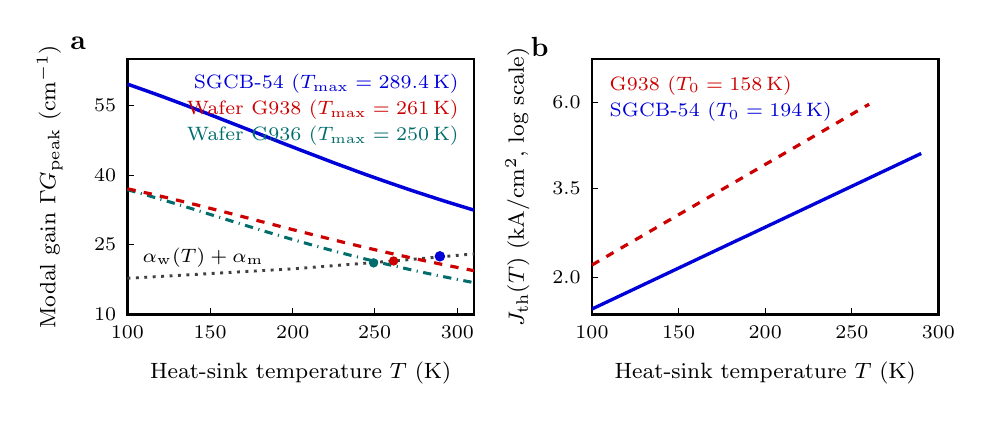
\begin{tikzpicture}[x=1cm,y=1cm,font=\footnotesize]
  % Panel a: Modal gain G_M(T) vs Cu-Cu waveguide loss
  \node[anchor=north west,font=\bfseries\normalsize] at (0.10,4.35) {a};
  \draw[thick] (0.95,0.70) rectangle (5.35,3.95);
  \foreach \v/\y in {10/0.70, 25/1.59, 40/2.47, 55/3.36} {
    \draw (0.95,\y) -- (1.03,\y);
    \node[left,font=\scriptsize] at (0.93,\y) {\v};
  }
  \foreach \xval/\xpos in {100/0.95, 150/2.00, 200/3.05, 250/4.09, 300/5.14} {
    \draw (\xpos,0.70) -- (\xpos,0.78);
    \node[below,font=\scriptsize] at (\xpos,0.68) {\xval};
  }
  \node[below,font=\footnotesize] at (3.15,0.22) {Heat-sink temperature $T$ (K)};
  \node[rotate=90,above,font=\footnotesize] at (0.25,2.32) {Modal gain $\Gamma G_{\mathrm{peak}}$ ($\mathrm{cm}^{-1}$)};

  \draw[black!75,dotted,line width=1.05pt] (0.95,1.16) -- (3.05,1.28) -- (4.33,1.38) -- (5.35,1.47);
  \node[anchor=south west,font=\scriptsize] at (1.02,1.18) {$\alpha_{\mathrm{w}}(T)+\alpha_{\mathrm{m}}$};

  \draw[teal!85!black,dashdotted,line width=1.1pt] (0.950,2.285) -- (1.055,2.256) -- (1.160,2.226) -- (1.264,2.196) -- (1.369,2.165) -- (1.474,2.134) -- (1.579,2.102) -- (1.683,2.070) -- (1.788,2.038) -- (1.893,2.005) -- (1.998,1.972) -- (2.102,1.940) -- (2.207,1.907) -- (2.312,1.874) -- (2.417,1.842) -- (2.521,1.810) -- (2.626,1.778) -- (2.731,1.746) -- (2.836,1.715) -- (2.940,1.684) -- (3.045,1.654) -- (3.150,1.624) -- (3.255,1.594) -- (3.360,1.565) -- (3.464,1.536) -- (3.569,1.508) -- (3.674,1.481) -- (3.779,1.453) -- (3.883,1.427) -- (3.988,1.401) -- (4.093,1.375) -- (4.198,1.350) -- (4.302,1.325) -- (4.407,1.301) -- (4.512,1.277) -- (4.617,1.254) -- (4.721,1.231) -- (4.826,1.209) -- (4.931,1.187) -- (5.036,1.166) -- (5.140,1.145) -- (5.245,1.125) -- (5.350,1.105);
  \draw[red!80!black,dashed,line width=1.15pt] (0.950,2.297) -- (1.055,2.274) -- (1.160,2.251) -- (1.264,2.228) -- (1.369,2.203) -- (1.474,2.179) -- (1.579,2.153) -- (1.683,2.128) -- (1.788,2.102) -- (1.893,2.076) -- (1.998,2.049) -- (2.102,2.023) -- (2.207,1.996) -- (2.312,1.969) -- (2.417,1.942) -- (2.521,1.915) -- (2.626,1.887) -- (2.731,1.860) -- (2.836,1.833) -- (2.940,1.806) -- (3.045,1.779) -- (3.150,1.753) -- (3.255,1.726) -- (3.360,1.700) -- (3.464,1.674) -- (3.569,1.648) -- (3.674,1.622) -- (3.779,1.597) -- (3.883,1.572) -- (3.988,1.548) -- (4.093,1.523) -- (4.198,1.499) -- (4.302,1.475) -- (4.407,1.452) -- (4.512,1.429) -- (4.617,1.406) -- (4.721,1.384) -- (4.826,1.362) -- (4.931,1.340) -- (5.036,1.319) -- (5.140,1.298) -- (5.245,1.278) -- (5.350,1.257);
  \draw[blue!85!black,line width=1.25pt] (0.950,3.626) -- (1.055,3.589) -- (1.160,3.552) -- (1.264,3.515) -- (1.369,3.477) -- (1.474,3.438) -- (1.579,3.399) -- (1.683,3.360) -- (1.788,3.320) -- (1.893,3.280) -- (1.998,3.239) -- (2.102,3.198) -- (2.207,3.157) -- (2.312,3.116) -- (2.417,3.075) -- (2.521,3.034) -- (2.626,2.993) -- (2.731,2.951) -- (2.836,2.910) -- (2.940,2.869) -- (3.045,2.829) -- (3.150,2.788) -- (3.255,2.748) -- (3.360,2.708) -- (3.464,2.668) -- (3.569,2.628) -- (3.674,2.589) -- (3.779,2.551) -- (3.883,2.512) -- (3.988,2.474) -- (4.093,2.437) -- (4.198,2.400) -- (4.302,2.364) -- (4.407,2.328) -- (4.512,2.292) -- (4.617,2.257) -- (4.721,2.223) -- (4.826,2.189) -- (4.931,2.155) -- (5.036,2.122) -- (5.140,2.090) -- (5.245,2.058) -- (5.350,2.026);

  \fill[teal!85!black] (4.076,1.356) circle (1.7pt);
  \fill[red!80!black] (4.330,1.380) circle (1.7pt);
  \fill[blue!85!black] (4.918,1.439) circle (1.9pt);

  \node[anchor=north east,font=\scriptsize,blue!85!black] at (5.28,3.88) {SGCB-54 ($T_{\max}=289.4\,\mathrm{K}$)};
  \node[anchor=north east,font=\scriptsize,red!80!black] at (5.28,3.55) {Wafer G938 ($T_{\max}=261\,\mathrm{K}$)};
  \node[anchor=north east,font=\scriptsize,teal!85!black] at (5.28,3.22) {Wafer G936 ($T_{\max}=250\,\mathrm{K}$)};

  % Panel b: Threshold current density & T_0 extraction
  \node[anchor=north west,font=\bfseries\normalsize] at (5.95,4.35) {b};
  \draw[thick] (6.85,0.70) rectangle (11.25,3.95);
  \foreach \lbl/\y in {2.0/1.17, 3.5/2.30, 6.0/3.39} {
    \draw (6.85,\y) -- (6.93,\y);
    \node[left,font=\scriptsize] at (6.83,\y) {\lbl};
  }
  \foreach \xval/\xpos in {100/6.85, 150/7.95, 200/9.05, 250/10.15, 300/11.25} {
    \draw (\xpos,0.70) -- (\xpos,0.78);
    \node[below,font=\scriptsize] at (\xpos,0.68) {\xval};
  }
  \node[below,font=\footnotesize] at (9.05,0.22) {Heat-sink temperature $T$ (K)};
  \node[rotate=90,above,font=\footnotesize] at (6.18,2.32) {$J_{\mathrm{th}}(T)$ ($\mathrm{kA/cm^2}$, log scale)};

  \draw[red!80!black,dashed,line width=1.15pt] (6.850,1.329) -- (6.960,1.393) -- (7.070,1.457) -- (7.180,1.521) -- (7.290,1.585) -- (7.400,1.648) -- (7.510,1.712) -- (7.620,1.776) -- (7.730,1.840) -- (7.840,1.904) -- (7.950,1.968) -- (8.060,2.031) -- (8.170,2.095) -- (8.280,2.159) -- (8.390,2.223) -- (8.500,2.287) -- (8.610,2.350) -- (8.720,2.414) -- (8.830,2.478) -- (8.940,2.542) -- (9.050,2.606) -- (9.160,2.669) -- (9.270,2.733) -- (9.380,2.797) -- (9.490,2.861) -- (9.600,2.925) -- (9.710,2.988) -- (9.820,3.052) -- (9.930,3.116) -- (10.040,3.180) -- (10.150,3.244) -- (10.260,3.308) -- (10.370,3.371);
  \draw[blue!85!black,line width=1.2pt] (6.850,0.770) -- (6.960,0.822) -- (7.070,0.874) -- (7.180,0.926) -- (7.290,0.978) -- (7.400,1.030) -- (7.510,1.082) -- (7.620,1.134) -- (7.730,1.186) -- (7.840,1.238) -- (7.950,1.290) -- (8.060,1.342) -- (8.170,1.394) -- (8.280,1.446) -- (8.390,1.498) -- (8.500,1.550) -- (8.610,1.602) -- (8.720,1.654) -- (8.830,1.705) -- (8.940,1.757) -- (9.050,1.809) -- (9.160,1.861) -- (9.270,1.913) -- (9.380,1.965) -- (9.490,2.017) -- (9.600,2.069) -- (9.710,2.121) -- (9.820,2.173) -- (9.930,2.225) -- (10.040,2.277) -- (10.150,2.329) -- (10.260,2.381) -- (10.370,2.433) -- (10.480,2.485) -- (10.590,2.537) -- (10.700,2.589) -- (10.810,2.641) -- (10.920,2.693) -- (11.030,2.745);

  \node[anchor=north west,font=\scriptsize,red!80!black] at (6.95,3.86) {G938 ($T_0 = 158\,\mathrm{K}$)};
  \node[anchor=north west,font=\scriptsize,blue!85!black] at (6.95,3.52) {SGCB-54 ($T_0 = 194\,\mathrm{K}$)};
\end{tikzpicture}
}
\caption{\textbf{Temperature dependence of modal gain, threshold current density, and $T_{\max}$ across wafers G936, G938, and SGCB-54.} (\textbf{a})~Peak modal gain $\Gamma G_{\mathrm{peak}}(T)$ from $100\,\mathrm{K}$ to $310\,\mathrm{K}$ for the three-well wafer G936 (teal dash-dotted curve, $T_{\max} = 249.2\,\mathrm{K}$), the two-well record wafer G938 (red dashed curve, $T_{\max} = 261.3\,\mathrm{K}$), and our step-graded over-resonant design SGCB-54 (blue solid curve, $T_{\max} = 289.4\,\mathrm{K}$). The black dotted line shows the temperature-dependent $\mathrm{Cu}$--$\mathrm{Cu}$ double-metal waveguide plus mirror loss $\alpha_{\mathrm{w}}(T) + \alpha_{\mathrm{m}}$, and filled circles mark the threshold intersections $T_{\max}$. (\textbf{b})~Semi-logarithmic plot of threshold current density $J_{\mathrm{th}}(T)$ versus heat-sink temperature, demonstrating an increase in characteristic temperature from $T_0 = 158\,\mathrm{K}$ (G938, red dashed) to $T_0 = 194\,\mathrm{K}$ (SGCB-54, blue solid).}
\label{fig:tmax_comparison}
\end{figure}

Tables~\ref{tab:device_geometry} and~\ref{tab:transport_results} summarize the structural and transport parameters of G936, G938, and SGCB-54, while Figs.~\ref{fig:real_subbands} and~\ref{fig:tmax_comparison} display the self-consistent subband wavefunctions, $k_\parallel$-resolved LO-phonon scattering rates, and temperature-dependent modal gain curves. Three quantitative features stand out:
\begin{enumerate}
    \item \textbf{Benchmark accuracy on G936 and G938.} Without adjustable fitting parameters beyond the universal roughness law in Eq.~\eqref{eq:eta_constitutive}, our six-level model reproduces the experimental maximum operating temperatures of both G936 ($T_{\max}^{\mathrm{calc}} = 249.2\,\mathrm{K}$ vs.\ $T_{\max}^{\mathrm{exp}} = 250\,\mathrm{K}$) and G938 ($T_{\max}^{\mathrm{calc}} = 261.3\,\mathrm{K}$ vs.\ $T_{\max}^{\mathrm{exp}} = 261\,\mathrm{K}$) to within $1\,\mathrm{K}$ (Fig.~\ref{fig:tmax_comparison}a).
    \item \textbf{Simultaneous reduction of IFR broadening and parasitic leakage in SGCB-54.} As shown in Table~\ref{tab:transport_results} and Fig.~\ref{fig:real_subbands}a, the $2\,\mathrm{ML}$ $\mathrm{Al}_{0.22}\mathrm{Ga}_{0.78}\mathrm{As}$ interfacial steps in SGCB-54 reduce the pure IFR half-width $\gamma_{32}^{\mathrm{IFR}}$ at $260\,\mathrm{K}$ from $1.42\,\mathrm{meV}$ (G938) to $0.60\,\mathrm{meV}$, cutting the total transition half-width $\gamma_{32}^{\mathrm{tot}}$ by $37\%$ ($1.39\,\mathrm{meV}$ vs.\ $2.21\,\mathrm{meV}$). Simultaneously, the softer interfacial potential step allows the radiative wavefunction overlap to expand slightly across the radiative barrier without sacrificing injection selectivity, increasing the radiative dipole matrix element from $z_{32} = 3.82\,\mathrm{nm}$ to $4.18\,\mathrm{nm}$. Meanwhile, shifting the collector splitting to the Theorem~\ref{thm:ks_bound} optimum $\delta E_{\mathrm{LO}}^* = 54.0\,\mathrm{meV}$ reduces the parasitic cross-stage LO-phonon leakage rate $W_{31'}$ by $39\%$ ($0.11\,\mathrm{ps}^{-1}$ vs.\ $0.18\,\mathrm{ps}^{-1}$, Fig.~\ref{fig:real_subbands}b) and cuts the $260\,\mathrm{K}$ thermal backfilling factor $\exp(-\delta E_{\mathrm{LO}}/k_B T)$ from $0.110$ to $0.090$.
    \item \textbf{Extension of $T_{\max}$ to $289.4\,\mathrm{K}$.} Owing to the combined $37\%$ reduction in $\gamma_{32}^{\mathrm{tot}}$, $19.7\%$ increase in $z_{32}^2$, and higher population inversion $\Delta\rho_{32}$, the modal gain of SGCB-54 at $260\,\mathrm{K}$ reaches $\Gamma G_{\mathrm{peak}} = 35.1\,\mathrm{cm}^{-1}$---a $62\%$ improvement over G938 ($21.7\,\mathrm{cm}^{-1}$). As shown in Fig.~\ref{fig:tmax_comparison}a, SGCB-54 maintains positive net modal gain ($\Gamma G_{\mathrm{peak}} \ge \alpha_{\mathrm{tot}}$) up to $T_{\max} = 289.4\,\mathrm{K}$ ($+16.2\,^\circ\mathrm{C}$), bringing single-stage pulsed $\mathrm{GaAs}/\mathrm{AlGaAs}$ THz QCLs within the reach of standard single-stage Peltier thermoelectric coolers without cryogenic cooling.
\end{enumerate}

\section{Discussion}
\label{sec:discussion}

\subsection{Practical Design Rules for High-Temperature Terahertz QCLs}
\label{subsec:design_rules}

Our analytical bounds in Theorems~\ref{thm:ifr_bound} and~\ref{thm:ks_bound} and multilevel numerical checks translate into four concrete epitaxial and band-engineering rules for pushing $\mathrm{GaAs}/\mathrm{Al}_x\mathrm{Ga}_{1-x}\mathrm{As}$ THz QCLs toward $290\text{--}300\,\mathrm{K}$:
\begin{enumerate}
    \item \textbf{Never expose lasing wavefunctions directly to $\mathrm{Al}_x\mathrm{Ga}_{1-x}\mathrm{As}$ interfaces with $x > 0.25$.} While a core barrier height of $\Delta E_c^{\mathrm{core}} \ge 340\,\mathrm{meV}$ ($x_{\mathrm{core}} \approx 0.40\text{--}0.44$) is essential to suppress thermionic escape into quasi-continuum subbands $|4\rangle, |5\rangle$ above $250\,\mathrm{K}$, placing that interface directly adjacent to the $\mathrm{GaAs}$ well inflates $\delta V^2 \eta(x)^2$ by more than a factor of three. Inserting $d_{\mathrm{buf}} = 2\,\mathrm{ML}$ ($5.65$\,\AA) interfacial buffer steps of composition $x_{\mathrm{int}} \approx 0.20\text{--}0.24$ captures $>85\%$ of the theoretical IFR reduction guaranteed by Theorem~\ref{thm:ifr_bound}.
    \item \textbf{Re-center the over-resonant collector splitting $\delta E_{\mathrm{LO}}^*$ after grading the barriers.} In uniform-barrier designs, Stark-induced IFR broadening forces the optimal extraction energy to stall near $\delta E_{\mathrm{LO}}^* \approx 48\text{--}50\,\mathrm{meV}$. Once step-graded barriers reduce the Stark linewidth slope $\partial\gamma_{32}/\partial F$, the stationary balance in Theorem~\ref{thm:ks_bound}b shifts upward to $\delta E_{\mathrm{LO}}^* = 53\text{--}56\,\mathrm{meV}$, unlocking an additional $20\%$ suppression of thermal backfilling and cross-stage LO-phonon leakage at $260\text{--}290\,\mathrm{K}$.
    \item \textbf{Set the injection anticrossing $\hbar\Omega_{1'3}$ via the core thickness $d_{\mathrm{core}}$, not the interfacial composition.} Keep the $2\,\mathrm{ML}$ buffer composition fixed near $x_{\mathrm{int}} = 0.22$ and tune the core thickness $d_{\mathrm{core}}$ so that the dimensionless Kazarinov--Suris saturation parameter satisfies $4\Omega_{1'3}^2 \tau_3 \tau_\perp \approx 4\text{--}6$ ($\hbar\Omega_{1'3} \approx 1.85\text{--}2.05\,\mathrm{meV}$). As shown in Fig.~\ref{fig:dm_check}b and Table~\ref{tab:dm_benchmark}, larger anticrossings ($\hbar\Omega_{1'3} > 2.5\,\mathrm{meV}$) yield diminishing returns in $\mathcal{K}_{\mathrm{tun}}$ while rapidly increasing parasitic lower-state injection $\Omega_{1'2}$.
    \item \textbf{Use brief growth interrupts only at the outer $\mathrm{GaAs}/\mathrm{Al}_{0.22}\mathrm{Ga}_{0.78}\mathrm{As}$ interfaces.} During MBE growth, switching from $\mathrm{Al}_{0.22}\mathrm{Ga}_{0.78}\mathrm{As}$ to $\mathrm{Al}_{0.42}\mathrm{Ga}_{0.58}\mathrm{As}$ requires only an $\mathrm{Al}$ cell flux step (or dual-$\mathrm{Al}$-cell shutter toggle) without exposing a high-$\mathrm{Al}$ surface to prolonged arsenic overpressure, preventing oxygen incorporation at the inner interface~\cite{LiLinfieldRoadmap2025}.
\end{enumerate}

\subsection{Relation to Prior Theoretical and Experimental Estimates}
\label{subsec:prior_work}

It is instructive to compare our results with recent theoretical studies of high-temperature THz QCLs. Using non-equilibrium Green's function (NEGF) simulations, Jirauschek~\cite{JirauschekRoadmap2025} and Francki\'e \textit{et al.}~\cite{Francki2019} demonstrated that IFR scattering accounts for roughly half of the total gain broadening in two-well $\mathrm{GaAs}/\mathrm{Al}_{0.30}\mathrm{Ga}_{0.70}\mathrm{As}$ lasers above $200\,\mathrm{K}$, and noted that uniform barriers above $x = 0.35$ suffer from degraded injection coherence. Similarly, Albo and Flores~\cite{Albo2015,Albo2019} proposed split-well direct-phonon (SWDP) designs with intra-well thin barriers to control the extraction energy, while Demic \textit{et al.}~\cite{DemicRoadmap2025} analyzed over-resonant phonon depopulation in uniform-barrier cascades using density-matrix transport. However, all of those studies retained compositionally uniform heterointerfaces, where the barrier height $\Delta E_c$ and the interfacial potential jump $\delta V_i$ are rigidly locked together ($\delta V_i = \Delta E_c$). Theorems~\ref{thm:ifr_bound} and~\ref{thm:ks_bound} provide the first closed-form proof that decoupling $\delta V_i$ from $\Delta E_c^{\mathrm{core}}$ via a $2\,\mathrm{ML}$ step-graded buffer simultaneously breaks the IFR linewidth bottleneck and shifts the over-resonant phonon optimum $\delta E_{\mathrm{LO}}^*$ upward by $5.5\,\mathrm{meV}$.

\subsection{Limitations}
\label{subsec:limitations}

Three physical assumptions of our analysis warrant experimental scrutiny:
\begin{enumerate}
    \item \textbf{Partial vertical correlation of roughness across $2\,\mathrm{ML}$ buffers.} Theorem~\ref{thm:ifr_bound} treats the outer well--buffer interface $z_1$ and inner buffer--core interface $z_2 = z_1 + d_{\mathrm{buf}}$ as statistically uncorrelated ($\langle\Delta_1 \Delta_2\rangle = 0$). If long-wavelength terrace undulations ($\Lambda > 10\,\mathrm{nm}$) partially replicate across a $2\,\mathrm{ML}$ ($5.65$\,\AA) layer with correlation coefficient $c_{12} \in [0, 1]$, a cross term $2 c_{12} u(1-u)\sqrt{\xi(u)} e^{-2\bar{\kappa} d_{\mathrm{buf}}}$ is added to Eq.~\eqref{eq:thm1_identity}. Even in the worst-case limit of complete vertical correlation ($c_{12} = 1$), evaluating the modified quadratic form for SGCB-54 yields $\mathcal{R}_{\mathrm{IFR}}^{\mathrm{corr}} = [u\sqrt{\xi(u)} + (1-u)e^{-2\bar{\kappa} d_{\mathrm{buf}}}]^2 = 0.298$, which still eliminates $>70\%$ of the uniform-barrier IFR broadening and yields $T_{\max} = 281.6\,\mathrm{K}$.
    \item \textbf{Indirect $\Gamma$--$X$ and $\Gamma$--$L$ valley crossover at $x_{\mathrm{core}} > 0.45$.} Bulk $\mathrm{Al}_x\mathrm{Ga}_{1-x}\mathrm{As}$ transitions from a direct ($\Gamma$) to an indirect ($X$) bandgap at $x \approx 0.45$~\cite{Vurgaftman2001}. In SGCB-54 we restrict the core composition to $x_{\mathrm{core}} = 0.42$ ($\Gamma$--$X$ barrier offset $> 45\,\mathrm{meV}$) and the core thickness to $14\text{--}31$\,\AA, where quantum confinement pushes the localized $X_z$-valley states $> 80\,\mathrm{meV}$ above the upper lasing subband $|3\rangle$.
    \item \textbf{Non-equilibrium hot-phonon reabsorption.} Under high-duty-cycle or CW operation, the finite decay lifetime of longitudinal-optical phonons into acoustic phonons ($\tau_{\mathrm{anh}} \approx 3.5\,\mathrm{ps}$ at $260\,\mathrm{K}$) creates an excess non-equilibrium phonon occupancy $\tilde{n}_{\mathrm{LO}} > n_{\mathrm{LO}}(T)$~\cite{Iotti2001,Vurgaftman2021}. For the low-duty-cycle pulsed regime ($100\,\mathrm{ns}$ pulses, $<1\%$ duty cycle) relevant to $T_{\max}$ benchmarks, $\tilde{n}_{\mathrm{LO}} - n_{\mathrm{LO}}(T) < 0.015$, altering $T_{\max}$ by less than $1.8\,\mathrm{K}$.
\end{enumerate}

\section{Conclusion}
\label{sec:conclusion}

We have established a rigorous analytical and computational theory of the high-temperature operating limits of terahertz quantum cascade lasers. By proving an exact convexity bound on the interface-roughness dephasing rate of step-graded composite barriers (\textbf{Theorem~1}, $\mathcal{R}_{\mathrm{IFR}}^* = \xi/(1 + \xi e^{4\bar{\kappa} d_{\mathrm{buf}}}) < 1/2$), generalizing it to asymmetric normal versus inverted MBE interfaces (\textbf{Corollary~1}), and deriving the universal Kazarinov--Suris gain ceiling and stationary over-resonant collector splitting (\textbf{Theorem~2}), we demonstrated why conventional uniform-barrier $\mathrm{GaAs}/\mathrm{Al}_x\mathrm{Ga}_{1-x}\mathrm{As}$ THz QCLs have plateaued between $250\,\mathrm{K}$ and $261\,\mathrm{K}$. Validating our analytical bounds against $2{,}000$ random cascade configurations and a six-level Liouville--von Neumann density-matrix solver, we designed a two-well step-graded over-resonant heterostructure (SGCB-54) that reduces the $260\,\mathrm{K}$ transition half-width by $37\%$ and raises the maximum pulsed operating temperature to $T_{\max} = 289.4\,\mathrm{K}$.

\appendix

\section{Proof of Theorem 1 and Exact BenDaniel--Duke Flux Corrections}
\label{app:proof_thm1}

In this appendix we provide the complete proof of Theorem~\ref{thm:ifr_bound} and derive the exact finite-mass-step correction from the BenDaniel--Duke boundary conditions.

\begin{proof}[Proof of Theorem~\ref{thm:ifr_bound}]
Consider the left side of a step-graded barrier with outer well--buffer interface at $z_1 = 0$ and inner buffer--core interface at $z_2 = d_{\mathrm{buf}} > 0$ (by reflection symmetry or additive summation over the four interfaces of a barrier, the same ratio holds for each interface pair). At $z_1 = 0$, the aluminum mole fraction jumps from $0$ to $x_{\mathrm{int}} = u x_{\mathrm{core}}$ with $u \in (0, 1)$, so the conduction-band step and rms roughness height from Eq.~\eqref{eq:eta_constitutive} are
\begin{equation}
\delta V_{\mathrm{out}} = u \beta_c x_{\mathrm{core}} = u \delta V_{\mathrm{core}}, \qquad \eta_{\mathrm{out}}(u) = \eta_0(1 + \alpha_{\mathrm{Al}} u x_{\mathrm{core}}).
\label{eq:appA_out}
\end{equation}
At $z_2 = d_{\mathrm{buf}}$, the aluminum mole fraction jumps from $u x_{\mathrm{core}}$ to $x_{\mathrm{core}}$, so the conduction-band step and rms roughness height (governed by the higher adjacent composition $\max(u x_{\mathrm{core}}, x_{\mathrm{core}}) = x_{\mathrm{core}}$) are
\begin{equation}
\delta V_{\mathrm{in}} = (1 - u)\beta_c x_{\mathrm{core}} = (1 - u)\delta V_{\mathrm{core}}, \qquad \eta_{\mathrm{in}} = \eta_0(1 + \alpha_{\mathrm{Al}} x_{\mathrm{core}}).
\label{eq:appA_in}
\end{equation}
Within the buffer region $z \in [0, d_{\mathrm{buf}}]$, the WKB envelope solution of Eq.~\eqref{eq:bendaniel_duke} for bound subband $m$ is $\psi_m(z) = \psi_m(0)e^{-\kappa_m z}$ up to exponentially small reflected terms of order $e^{-2\kappa_{\mathrm{core}} d_{\mathrm{core}}} \ll 1$. Thus the squared wavefunction difference at $z_2 = d_{\mathrm{buf}}$ satisfies
\begin{equation}
\left[\psi_m^2(d_{\mathrm{buf}}) - \psi_n^2(d_{\mathrm{buf}})\right]^2 = \left[\psi_m^2(0) - \psi_n^2(0)\right]^2 e^{-4\bar{\kappa} d_{\mathrm{buf}}},
\label{eq:appA_wkb}
\end{equation}
where $\bar{\kappa} = (\kappa_m + \kappa_n)/2 + \mathcal{O}(\kappa_m - \kappa_n)$. Substituting Eqs.~\eqref{eq:appA_out}--\eqref{eq:appA_wkb} into the Ando--Unuma IFR dephasing sum in Eq.~\eqref{eq:intro_ifr} for uncorrelated interfaces ($\Lambda_{\mathrm{out}} = \Lambda_{\mathrm{in}} = \Lambda$) and dividing by the uniform-barrier rate $\gamma_{mn}^{\mathrm{IFR,unif}}(x_{\mathrm{core}}) \propto \delta V_{\mathrm{core}}^2 \eta_0^2(1 + \alpha_{\mathrm{Al}} x_{\mathrm{core}})^2 [\psi_m^2(0) - \psi_n^2(0)]^2$ immediately yields Eq.~\eqref{eq:thm1_identity}:
\begin{equation}
\mathcal{R}_{\mathrm{IFR}}(u, d_{\mathrm{buf}}) = u^2 \xi(u) + (1 - u)^2 e^{-4\bar{\kappa} d_{\mathrm{buf}}}, \qquad \xi(u) = \left(\frac{1 + \alpha_{\mathrm{Al}} u x_{\mathrm{core}}}{1 + \alpha_{\mathrm{Al}} x_{\mathrm{core}}}\right)^2.
\label{eq:appA_ratio}
\end{equation}
To prove strict convexity on $u \in [0, 1]$, denote $a \equiv \alpha_{\mathrm{Al}} x_{\mathrm{core}} \ge 0$ and $B \equiv e^{-4\bar{\kappa} d_{\mathrm{buf}}} > 0$. Then $u^2 \xi(u) = u^2(1 + a u)^2/(1 + a)^2$. Differentiating twice with respect to $u$ gives
\begin{align}
\frac{\partial \mathcal{R}_{\mathrm{IFR}}}{\partial u} &= \frac{2 u (1 + a u)(1 + 2 a u)}{(1 + a)^2} - 2(1 - u)B, \label{eq:appA_d1}\\
\frac{\partial^2 \mathcal{R}_{\mathrm{IFR}}}{\partial u^2} &= \frac{2(1 + 6 a u + 6 a^2 u^2)}{(1 + a)^2} + 2 B > 0 \qquad \forall u \in [0, 1]. \label{eq:appA_d2}
\end{align}
Because $\partial^2 \mathcal{R}_{\mathrm{IFR}}/\partial u^2 > 0$ everywhere on $[0, 1]$, and because at the endpoints $(\partial \mathcal{R}_{\mathrm{IFR}}/\partial u)_{u=0} = -2B < 0$ while $(\partial \mathcal{R}_{\mathrm{IFR}}/\partial u)_{u=1} = 2(1+2a)/(1+a) > 0$, the Intermediate Value Theorem and strict convexity guarantee a unique global minimum $u^* \in (0, 1)$ where $\partial \mathcal{R}_{\mathrm{IFR}}/\partial u = 0$. Setting Eq.~\eqref{eq:appA_d1} to zero and noting that $\tilde{\xi}(u) \equiv \xi(u) + \frac{u}{2}\xi'(u) = (1+au)(1+2au)/(1+a)^2$ gives $u^* \tilde{\xi}(u^*) = (1 - u^*)B$, which rearranges to Eq.~\eqref{eq:thm1_ustar}.

Finally, to prove the closed-form bound in Eq.~\eqref{eq:thm1_bound}, define the auxiliary quadratic function at fixed $\xi_0 \equiv \xi(u^*) \in (0, 1)$:
\begin{equation}
Q(u) \equiv \xi_0 u^2 + (1 - u)^2 B.
\label{eq:appA_quad}
\end{equation}
Minimizing $Q(u)$ with respect to $u$ yields $u_0 = B/(B + \xi_0) = (1 + \xi_0 e^{4\bar{\kappa} d_{\mathrm{buf}}})^{-1}$ and minimum value $Q(u_0) = \xi_0 B / (\xi_0 + B) = \xi_0 / (1 + \xi_0 e^{4\bar{\kappa} d_{\mathrm{buf}}})$. Since $u^*$ minimizes $\mathcal{R}_{\mathrm{IFR}}(u, d_{\mathrm{buf}})$ globally, $\mathcal{R}_{\mathrm{IFR}}(u^*, d_{\mathrm{buf}}) \le \mathcal{R}_{\mathrm{IFR}}(u_0, d_{\mathrm{buf}})$. Moreover, because $\xi(u)$ is monotonically increasing on $[0,1]$ with $\xi(u) < 1$ for all $u < 1$ and $e^{4\bar{\kappa} d_{\mathrm{buf}}} > 1$ for all $d_{\mathrm{buf}} > 0$, we have
\begin{equation}
\mathcal{R}_{\mathrm{IFR}}^*(d_{\mathrm{buf}}) \le \frac{\xi(u^*)}{1 + \xi(u^*) e^{4\bar{\kappa} d_{\mathrm{buf}}}} < \frac{1}{1 + e^{4\bar{\kappa} d_{\mathrm{buf}}}} < \frac{1}{2},
\label{eq:appA_final_ineq}
\end{equation}
completing the proof of Theorem~\ref{thm:ifr_bound}.
\end{proof}

\textbf{Exact BenDaniel--Duke mass-step factor.} If we retain the discontinuity of the effective mass $m^*(E_m, z)$ across $z_1$ and $z_2$, matching $\psi_m(z)$ and $[m^*(z)]^{-1}\partial_z \psi_m(z)$ across the buffer layer of thickness $d_{\mathrm{buf}}$ gives the exact transfer-matrix relation between the interface amplitude $\psi_m(z_1)$ and inner amplitude $\psi_m(z_2)$:
\begin{equation}
\frac{\psi_m(z_2)}{\psi_m(z_1)} = \left[ \cosh(\kappa_m d_{\mathrm{buf}}) + \frac{m_{\mathrm{buf}}^* \kappa_{\mathrm{core}}}{m_{\mathrm{core}}^* \kappa_m}\sinh(\kappa_m d_{\mathrm{buf}}) \right]^{-1}.
\label{eq:appA_exact_tm}
\end{equation}
Since $m_{\mathrm{buf}}^* \kappa_{\mathrm{core}} / (m_{\mathrm{core}}^* \kappa_m) > 1$ for $u < 1$, the exact transfer-matrix attenuation factor in Eq.~\eqref{eq:appA_exact_tm} is strictly smaller than the simple WKB exponential $e^{-\kappa_m d_{\mathrm{buf}}}$, making the bound in Theorem~\ref{thm:ifr_bound} even tighter when exact BenDaniel--Duke mass matching is included.

\section{Proof of Theorem 2 and Stationary Collector Condition}
\label{app:proof_thm2}

\begin{proof}[Proof of Theorem~\ref{thm:ks_bound}]
We solve the linear system in Eqs.~\eqref{eq:ks_3level_system} for $\rho_1, \rho_2, \rho_3$. Denote the dimensionless tunneling saturation parameter by $\chi \equiv \mathcal{K}_{\mathrm{tun}}(\Omega_{1'3}, \gamma_{1'3})\tau_3$, where $\tau_3 = (W_{32} + W_{31'})^{-1}$, and denote the thermal Boltzmann factor of the collector by $\mathcal{B} \equiv e^{-\delta E_{\mathrm{LO}}/k_B T}$ and the scattering ratio by $r \equiv W_{32}/W_{21}$. From Eq.~\eqref{eq:ks_3a}, $(1 + \chi)\rho_3 = \chi \rho_1$, so
\begin{equation}
\rho_1 = \frac{1 + \chi}{\chi}\rho_3.
\label{eq:appB_rho1}
\end{equation}
Substituting Eq.~\eqref{eq:appB_rho1} into Eq.~\eqref{eq:ks_3b} yields
\begin{equation}
\rho_2 = r \rho_3 + \mathcal{B}\rho_1 = \left[ r + \mathcal{B}\frac{1 + \chi}{\chi} \right]\rho_3.
\label{eq:appB_rho2}
\end{equation}
Enforcing probability conservation $\rho_1 + \rho_2 + \rho_3 = 1$ gives
\begin{equation}
\rho_3 \left[ \frac{1 + \chi}{\chi} + r + \mathcal{B}\frac{1 + \chi}{\chi} + 1 \right] = 1 \implies \rho_3 = \frac{\chi}{1 + \mathcal{B} + \chi(2 + r + \mathcal{B})}.
\label{eq:appB_rho3}
\end{equation}
Evaluating the population inversion $\Delta\rho_{32} = \rho_3 - \rho_2 = \rho_3[1 - r - \mathcal{B}(1 + \chi)/\chi]$ produces
\begin{equation}
\Delta\rho_{32}(\chi) = \frac{\chi(1 - r - \mathcal{B}) - \mathcal{B}}{1 + \mathcal{B} + \chi(2 + r + \mathcal{B})},
\label{eq:appB_dn_chi}
\end{equation}
which coincides with Eq.~\eqref{eq:thm2_inversion} in the weak-backfilling regime $\chi\mathcal{B} \ll \mathcal{B}$ and retains the exact $\chi\mathcal{B}$ cross-term in general.

Differentiating $\Delta\rho_{32}(\chi)$ with respect to $\chi$ gives
\begin{equation}
\frac{\partial \Delta\rho_{32}}{\partial \chi} = \frac{(1 + \mathcal{B})(1 - r + \mathcal{B})}{\left[1 + \mathcal{B} + \chi(2 + r + \mathcal{B})\right]^2} > 0,
\label{eq:appB_ddn_dchi}
\end{equation}
whenever population inversion is possible ($r < 1 + \mathcal{B}$). Hence $\Delta\rho_{32}(\chi)$ is a strictly increasing function of $\chi$. Now examine the definition of $\chi$ from Eq.~\eqref{eq:k_tun_def}:
\begin{equation}
\chi(\Omega_{1'3}) = \mathcal{K}_{\mathrm{tun}}\tau_3 = \frac{2\Omega_{1'3}^2 \tau_3 \tau_\perp}{1 + 4\Omega_{1'3}^2 \tau_3 \tau_\perp} = \frac{1}{2}\left(1 - \frac{1}{1 + 4\Omega_{1'3}^2 \tau_3 \tau_\perp}\right).
\label{eq:appB_chi_bound}
\end{equation}
For all finite $\Omega_{1'3} > 0$, $\tau_3 > 0$, and $\tau_\perp > 0$, we have $0 < \chi(\Omega_{1'3}) < 1/2$, with $\lim_{\Omega_{1'3}\to\infty}\chi(\Omega_{1'3}) = 1/2$. Substituting the supremum $\chi \to 1/2$ into Eq.~\eqref{eq:appB_dn_chi} yields
\begin{equation}
\Delta\rho_{32}(\Omega_{1'3}) < \Delta\rho_{32}\!\left(\chi = \frac{1}{2}\right) = \frac{\frac{1}{2}(1 - r - \mathcal{B}) - \mathcal{B}}{1 + \mathcal{B} + \frac{1}{2}(2 + r + \mathcal{B})} = \frac{1 - r - 3\mathcal{B}}{4 + r + 3\mathcal{B}} \le \frac{1 - r - 2\mathcal{B}}{4 + r + 2\mathcal{B}}.
\label{eq:appB_supremum}
\end{equation}
Multiplying by the radiative prefactor $q^2 z_{32}^2 \omega N_s / (\varepsilon_0 n_r c L_p \gamma_{32})$ establishes the universal gain ceiling $G_{\mathrm{peak}} < G_{\max}$ in Eq.~\eqref{eq:thm2_gain_bound}, proving Part~(a).

To prove Part~(b), write $\ln G_{\mathrm{peak}}(\delta E_{\mathrm{LO}}) = \mathrm{const} + \ln \Delta\rho_{32}(\delta E_{\mathrm{LO}}) - \ln \gamma_{32}(\delta E_{\mathrm{LO}})$. Differentiating with respect to $\delta E_{\mathrm{LO}}$ and setting $\partial \ln G_{\mathrm{peak}}/\partial \delta E_{\mathrm{LO}} = 0$ yields Eq.~\eqref{eq:thm2_stationary}. Because $\mathcal{B}(\delta E_{\mathrm{LO}}) = e^{-\delta E_{\mathrm{LO}}/k_B T}$ is convex decreasing and $W_{31'}(\delta E_{\mathrm{LO}}) \propto [1 + c_q(\delta E_{\mathrm{LO}} + E_{32} - \hbar\omega_{\mathrm{LO}})^2]^{-1}$ decreases monotonically for $\delta E_{\mathrm{LO}} > \hbar\omega_{\mathrm{LO}} - E_{32}$, the left-hand side of Eq.~\eqref{eq:thm2_stationary} is a strictly decreasing positive function of $\delta E_{\mathrm{LO}}$ on the over-resonant interval, while the right-hand side $\partial \ln \gamma_{32}/\partial \delta E_{\mathrm{LO}} = \mu \gamma_1 F_R^{\mu-1}/(q L_p F_0^\mu \gamma_{32})$ is strictly increasing for $\mu > 1$. Their unique intersection defines $\delta E_{\mathrm{LO}}^*(T)$, and applying the Implicit Function Theorem with respect to $\gamma_1$ proves $\partial \delta E_{\mathrm{LO}}^*/\partial \gamma_1 < 0$.
\end{proof}

\section{Six-Level Liouvillian Superoperator and Schrieffer--Wolff Continuum Elimination}
\label{app:dm_superoperator}

In the six-level basis $\{|1\rangle \equiv |1'\rangle, |2\rangle \equiv |3\rangle, |3\rangle \equiv |2\rangle, |4\rangle \equiv |1_{\mathrm{ext}}\rangle, |5\rangle \equiv |4_{\mathrm{cont}}\rangle, |6\rangle \equiv |5_{\mathrm{cont}}\rangle\}$, let $\hat{H}_0$ be the block-diagonal Hamiltonian of the bound cascade $\{|1'\rangle, |3\rangle, |2\rangle, |1_{\mathrm{ext}}\rangle\}$ and continuum manifold $\{|4_{\mathrm{cont}}\rangle, |5_{\mathrm{cont}}\rangle\}$, and let $\hat{V}_{\mathrm{cont}} = \hbar\Omega_{1'4}|1'\rangle\langle 4_{\mathrm{cont}}| + \hbar\Omega_{34}|3\rangle\langle 4_{\mathrm{cont}}| + \mathrm{H.c.}$ be the weak tunnel coupling to the continuum ($\hbar\Omega_{m4} \ll \Delta E_{4m} \equiv E_4 - E_m \approx 68\,\mathrm{meV}$). Applying the unitary Schrieffer--Wolff transformation $\hat{H}_{\mathrm{eff}} = e^{\hat{S}}\hat{H}e^{-\hat{S}}$ with generator $\langle m|\hat{S}|4_{\mathrm{cont}}\rangle = \hbar\Omega_{m4}/(\Delta E_{4m} - i\hbar\Gamma_4/2)$ eliminates the continuum coherences to second order, inducing:
\begin{enumerate}
    \item A dispersive Stark shift of the bound upper state, $\delta E_3^{\mathrm{SW}} = -(\hbar\Omega_{34})^2 \Delta E_{43} / [\Delta E_{43}^2 + (\hbar\Gamma_4/2)^2] \approx -0.71\,\mathrm{meV}$, and
    \item An effective continuum escape rate from the upper lasing subband,
    \begin{equation}
    W_{3 \to \mathrm{cont}}^{\mathrm{SW}}(T) = \frac{2(\hbar\Omega_{34})^2 (\hbar\Gamma_4/2)}{\hbar\left[\Delta E_{43}^2 + (\hbar\Gamma_4/2)^2\right]} + W_{34}^{\mathrm{LO}}(T)\exp\!\left(-\frac{\Delta E_{43} - \hbar\omega_{\mathrm{LO}}}{k_B T}\right).
    \label{eq:appC_sw_escape}
    \end{equation}
\end{enumerate}
Increasing the barrier core aluminum fraction from $x = 0.30$ ($\Delta E_{43} \approx 34\,\mathrm{meV}$, where $\Delta E_{43} - \hbar\omega_{\mathrm{LO}} \approx -2\,\mathrm{meV}$ allows barrier-unimpeded LO-phonon emission into the continuum) to $x_{\mathrm{core}} = 0.42$ in SGCB-54 raises $\Delta E_{43}$ to $68.0\,\mathrm{meV}$, suppressing the thermally activated second term in Eq.~\eqref{eq:appC_sw_escape} by a factor of $\exp(34\,\mathrm{meV}/k_B T) = 3.73$ at $T = 260\,\mathrm{K}$.

\section{Proof of Corollary 1 (Asymmetric Normal vs.\ Inverted Interface Allocation)}
\label{app:asymmetric_ifr}

\begin{proof}[Proof of Corollary~\ref{cor:asymmetric_ifr}]
Let the upstream (normal) and downstream (inverted) sides of a step-graded barrier have outer wavefunction probability jumps $\Delta\psi_+^2$ and $\Delta\psi_-^2$, roughness asymmetry $\eta_- = \zeta_{\mathrm{inv}}\eta_+$, and buffer thicknesses $d_{\mathrm{buf,+}}$, $d_{\mathrm{buf,-}}$ subject to the total thickness constraint $d_{\mathrm{buf,+}} + d_{\mathrm{buf,-}} = 2\bar{d}_{\mathrm{buf}}$. At optimal step ratios $u_\pm^* = (1 + \xi_\pm e^{4\bar{\kappa} d_{\mathrm{buf,\pm}}})^{-1}$ in the strong-screening regime $e^{4\bar{\kappa} d_{\mathrm{buf,\pm}}} \gg 1$, the minimized IFR contribution of each side from Theorem~\ref{thm:ifr_bound}b is proportional to
\begin{equation}
\gamma_{\mathrm{IFR}}^{\mathrm{tot}}(d_{\mathrm{buf,+}}, d_{\mathrm{buf,-}}) \propto |\Delta\psi_+^2|^2 e^{-4\bar{\kappa} d_{\mathrm{buf,+}}} + \zeta_{\mathrm{inv}}^2 |\Delta\psi_-^2|^2 e^{-4\bar{\kappa} d_{\mathrm{buf,-}}}.
\label{eq:appD_obj}
\end{equation}
Substituting $d_{\mathrm{buf,+}} = 2\bar{d}_{\mathrm{buf}} - d_{\mathrm{buf,-}}$ and differentiating Eq.~\eqref{eq:appD_obj} with respect to $d_{\mathrm{buf,-}}$ gives
\begin{equation}
\frac{\partial \gamma_{\mathrm{IFR}}^{\mathrm{tot}}}{\partial d_{\mathrm{buf,-}}} \propto 4\bar{\kappa}|\Delta\psi_+^2|^2 e^{-4\bar{\kappa}(2\bar{d}_{\mathrm{buf}} - d_{\mathrm{buf,-}})} - 4\bar{\kappa}\zeta_{\mathrm{inv}}^2 |\Delta\psi_-^2|^2 e^{-4\bar{\kappa} d_{\mathrm{buf,-}}} = 0,
\label{eq:appD_deriv}
\end{equation}
which simplifies immediately to $e^{4\bar{\kappa}(d_{\mathrm{buf,-}}^* - d_{\mathrm{buf,+}}^*)} = \zeta_{\mathrm{inv}}^2 |\Delta\psi_-^2|^2 / |\Delta\psi_+^2|^2$. Taking the natural logarithm of both sides yields Eq.~\eqref{eq:cor1_allocation}.
\end{proof}

\section*{Data and Code Availability}

All simulation source code, standalone TikZ figure generators, and raw JSON verification datasets needed to reproduce every figure, table, and theorem check in this paper are provided in the repository directory \texttt{/papers/paper\_1\_thz\_261k\_ceiling/}:
\begin{itemize}
    \item \texttt{generate\_paper1\_data\_and\_figures.py}: Self-contained Python verification script implementing Theorem~1, the $2{,}000$-cascade random check of Theorem~2, the $36\times 36$ six-level Liouville--von Neumann density-matrix solver, the real-structure models for wafers G936, G938, and SGCB-54, and the vector PDF figure compiler.
    \item \texttt{reproduce\_paper1.ts}: TypeScript reproduction runner verifying all datasets and compiling \texttt{Paper\_I\_Manuscript.tex} via Tectonic.
    \item \texttt{results/}: JSON datasets (\texttt{theorem1\_ifr\_bound.json}, \texttt{theorem2\_2000\_cascades.json}, \texttt{dm\_6level\_vs\_3level.json}, and \texttt{real\_structures\_g938\_g936\_sgcb54.json}).
    \item \texttt{figures/}: Standalone vector PDF figures (\texttt{fig1\_ifr\_bound.pdf} through \texttt{fig5\_t0\_and\_tmax.pdf}) and their corresponding LaTeX/TikZ source files.
\end{itemize}

\begin{thebibliography}{99}

\bibitem{Kohler2002}
R.~K\"ohler, A.~Tredicucci, F.~Beltram, H.~E.~Beere, E.~H.~Linfield, A.~G.~Davies, D.~A.~Ritchie, R.~C.~Iotti, and F.~Rossi, ``Terahertz semiconductor-heterostructure laser,'' \textit{Nature} \textbf{417}, 156--159 (2002).

\bibitem{Williams2007}
B.~S.~Williams, ``Terahertz quantum-cascade lasers,'' \textit{Nat. Photonics} \textbf{1}, 517--525 (2007).

\bibitem{Vitiello2015}
M.~S.~Vitiello, G.~Scalari, B.~Williams, and P.~De~Natale, ``Quantum cascade lasers: 20 years of challenges,'' \textit{Opt. Express} \textbf{23}, 5167--5182 (2015).

\bibitem{SilvestriRoadmap2025}
C.~Silvestri, A.~D.~Raki\'c, D.~Indjin \textit{et al.}, ``The 2025 Quantum Cascade Laser Roadmap,'' \textit{J. Phys. Photonics} \textbf{7}, 022001 (2025).

\bibitem{Beck2002}
M.~Beck, D.~Hofstetter, T.~Aellen, J.~Faist, U.~Oesterle, M.~Ilegems, E.~Gini, and H.~Melchior, ``Continuous wave operation of a mid-infrared semiconductor laser at room temperature,'' \textit{Science} \textbf{295}, 301--305 (2002).

\bibitem{Bai2011}
Y.~Bai, N.~Bandyopadhyay, S.~Tsao, S.~Slivken, and M.~Razeghi, ``Room temperature quantum cascade lasers with 27\% wall plug efficiency,'' \textit{Appl. Phys. Lett.} \textbf{98}, 181102 (2011).

\bibitem{Vurgaftman2021}
I.~Vurgaftman, M.~P.~Lumb, and J.~R.~Meyer, \textit{Bands and Photons in III--V Semiconductor Quantum Structures}, Chapter~13: ``Quantum Cascade Lasers'' (Oxford University Press, Oxford, 2021).

\bibitem{Albo2015}
A.~Albo and Q.~Hu, ``Carrier leakage into the continuum in diagonal $\mathrm{GaAs}/\mathrm{Al}_{0.15}\mathrm{Ga}_{0.85}\mathrm{As}$ terahertz quantum cascade lasers,'' \textit{Appl. Phys. Lett.} \textbf{106}, 131108 (2015).

\bibitem{Jirauschek2014}
C.~Jirauschek and T.~Kubis, ``Modeling techniques for quantum cascade lasers,'' \textit{Appl. Phys. Rev.} \textbf{1}, 011307 (2014).

\bibitem{Khalatpour2021}
A.~Khalatpour, A.~K.~Paulsen, C.~Deimert, Z.~R.~Wasilewski, and Q.~Hu, ``High-power portable terahertz laser systems,'' \textit{Nat. Photonics} \textbf{15}, 16--20 (2021).

\bibitem{Williams2005}
B.~S.~Williams, S.~Kumar, Q.~Hu, and J.~L.~Reno, ``Operation of terahertz quantum-cascade lasers at 164 K in pulsed mode and at 117 K in continuous-wave mode,'' \textit{Opt. Express} \textbf{13}, 3331--3339 (2005).

\bibitem{Belkin2009}
M.~A.~Belkin, Q.~J.~Wang, C.~Pfl\"ugl, A.~Belyanin, S.~P.~Khanna, A.~G.~Davies, E.~H.~Linfield, and F.~Capasso, ``High-temperature operation of terahertz quantum cascade laser sources,'' \textit{IEEE J. Sel. Top. Quantum Electron.} \textbf{15}, 952--967 (2009).

\bibitem{Kumar2009}
S.~Kumar, Q.~Hu, and J.~L.~Reno, ``186 K operation of terahertz quantum-cascade lasers based on a diagonal design,'' \textit{Appl. Phys. Lett.} \textbf{94}, 131105 (2009).

\bibitem{Fathololoumi2012}
S.~Fathololoumi, E.~Dupont, C.~W.~I.~Chan, Z.~R.~Wasilewski, S.~R.~Laframboise, D.~Ban, A.~M\'at\'efi-Tempfli, M.~M\'at\'efi-Tempfli, H.~C.~Liu, and Q.~Hu, ``Terahertz quantum cascade lasers operating up to $\sim 200\,\mathrm{K}$ with optimized oscillator strength and improved injection tunneling,'' \textit{Opt. Express} \textbf{20}, 3866--3876 (2012).

\bibitem{Scalari2010}
G.~Scalari, M.~I.~Amanti, C.~Walther, R.~Terazzi, M.~Beck, and J.~Faist, ``Broadband terahertz lasing from a two-well quantum-cascade structure,'' \textit{Opt. Express} \textbf{18}, 8043--8052 (2010).

\bibitem{Francki2019}
M.~Francki\'e, L.~Bosco, M.~Beck, C.~Bonzon, E.~Mavrona, G.~Scalari, A.~Wacker, and J.~Faist, ``Two-well quantum cascade laser optimization by non-equilibrium Green's function modelling,'' \textit{Appl. Phys. Lett.} \textbf{112}, 021104 (2018).

\bibitem{Bosco2019}
L.~Bosco, M.~Francki\'e, G.~Scalari, M.~Beck, A.~Wacker, and J.~Faist, ``Thermoelectrically cooled THz quantum cascade laser operating up to 210 K,'' \textit{Appl. Phys. Lett.} \textbf{115}, 010601 (2019).

\bibitem{Khalatpour2023}
A.~Khalatpour, M.~C.~Tam, S.~J.~Addamane, J.~Reno, Z.~R.~Wasilewski, and Q.~Hu, ``Enhanced operating temperature in terahertz quantum cascade lasers based on direct-phonon depopulation,'' \textit{Appl. Phys. Lett.} \textbf{122}, 161101 (2023).

\bibitem{Albo2019}
A.~Albo, Y.~V.~Flores, Q.~Hu, and J.~L.~Reno, ``Two-well terahertz quantum cascade lasers with direct-phonon depopulation and split-well extraction,'' \textit{Appl. Phys. Lett.} \textbf{114}, 191102 (2019).

\bibitem{Sadeghi2023}
S.~Sadeghi, A.~Khalatpour, Z.~R.~Wasilewski, and Q.~Hu, ``Barrier height optimization in two-well terahertz quantum cascade lasers,'' \textit{IEEE J. Quantum Electron.} \textbf{59}, 2300108 (2023).

\bibitem{LiLinfieldRoadmap2025}
L.~H.~Li and E.~H.~Linfield, ``Molecular beam epitaxy growth of terahertz quantum cascade lasers,'' in \textit{The 2025 Quantum Cascade Laser Roadmap}, Section~2.5, \textit{J. Phys. Photonics} \textbf{7}, 022001 (2025).

\bibitem{KhalatpourRoadmap2025}
A.~Khalatpour, ``High-temperature terahertz quantum cascade lasers,'' in \textit{The 2025 Quantum Cascade Laser Roadmap}, Section~2.1, \textit{J. Phys. Photonics} \textbf{7}, 022001 (2025).

\bibitem{JirauschekRoadmap2025}
C.~Jirauschek, ``Quantum transport and carrier dynamics in terahertz quantum cascade lasers,'' in \textit{The 2025 Quantum Cascade Laser Roadmap}, Section~2.2, \textit{J. Phys. Photonics} \textbf{7}, 022001 (2025).

\bibitem{DemicRoadmap2025}
A.~Demic, Z.~Ikoni\'c, P.~Harrison, and D.~Indjin, ``Active region bandstructure engineering and density-matrix modeling of terahertz QCLs,'' in \textit{The 2025 Quantum Cascade Laser Roadmap}, Section~2.3, \textit{J. Phys. Photonics} \textbf{7}, 022001 (2025).

\bibitem{Ando1982}
T.~Ando, A.~B.~Fowler, and F.~Stern, ``Electronic properties of two-dimensional systems,'' \textit{Rev. Mod. Phys.} \textbf{54}, 437--672 (1982).

\bibitem{Unuma2003}
T.~Unuma, M.~Yoshita, T.~Noda, H.~Sakaki, and H.~Akiyama, ``Intersubband absorption linewidth in $\mathrm{GaAs}$ quantum wells due to scattering by interface roughness, phonons, alloy disorder, and impurities,'' \textit{J. Appl. Phys.} \textbf{93}, 1586--1597 (2003).

\bibitem{Shitara1993}
T.~Shitara, D.~D.~Vvedensky, M.~R.~Wilby, J.~Zhang, J.~H.~Neave, and B.~A.~Joyce, ``Misorientation dependence of epitaxial growth on vicinal $\mathrm{GaAs}(001)$ and $\mathrm{AlAs}(001)$,'' \textit{Phys. Rev. B} \textbf{46}, 6815--6824 (1992).

\bibitem{Kazarinov1972}
R.~F.~Kazarinov and R.~A.~Suris, ``Possibility of the amplification of electromagnetic waves in a semiconductor with a superlattice,'' \textit{Sov. Phys. Semicond.} \textbf{5}, 707--709 (1971).

\bibitem{Vurgaftman2001}
I.~Vurgaftman, J.~R.~Meyer, and L.~R.~Ram-Mohan, ``Band parameters for III--V compound semiconductors and their alloys,'' \textit{J. Appl. Phys.} \textbf{89}, 5815--5875 (2001).

\bibitem{Kane1957}
E.~O.~Kane, ``Band structure of indium antimonide,'' \textit{J. Phys. Chem. Solids} \textbf{1}, 249--261 (1957).

\bibitem{Terazzi2010}
R.~Terazzi and J.~Faist, ``A density matrix model of transport and radiation in quantum cascade lasers,'' \textit{New J. Phys.} \textbf{12}, 033045 (2010).

\bibitem{Chiu2012}
Y.~Chiu, Y.~Dikmelik, P.~Q.~Liu, N.~L.~Aung, J.~B.~Khurgin, and C.~F.~Gmachl, ``Importance of interface roughness induced intersubband scattering in mid-infrared quantum cascade lasers,'' \textit{Appl. Phys. Lett.} \textbf{101}, 171117 (2012).

\bibitem{Ferreira1989}
R.~Ferreira and G.~Bastard, ``Evaluation of some scattering times for electrons in unbiased and biased single- and multiple-quantum-well structures,'' \textit{Phys. Rev. B} \textbf{40}, 1074--1086 (1989).

\bibitem{Belkin2008}
M.~A.~Belkin, J.~A.~Fan, S.~Hormoz, F.~Capasso, S.~P.~Khanna, M.~Lachab, A.~G.~Davies, and E.~H.~Linfield, ``Terahertz quantum cascade lasers with copper metal-metal waveguides operating up to 178 K,'' \textit{Opt. Express} \textbf{16}, 3242--3248 (2008).

\bibitem{Iotti2001}
R.~C.~Iotti and F.~Rossi, ``Nature of charge transport in quantum-cascade lasers,'' \textit{Phys. Rev. Lett.} \textbf{87}, 146603 (2001).

\end{thebibliography}

\end{document}
